\chapter{Fitting in the light of LHC data}
\label{ch:LHClight}
The addition of the first LHC datasets into an NNPDF fit allowed for important gains to be made in the precision of the resulting sets. However the potential dataset available for PDF determination from the LHC is increasing at a considerable rate, and datasets are being rapidly updated with more precise measurements. There is therefore still much more potential in the LHC to provide PDF constraint, especially in collider only fits.

With the ever enlarging dataset comes an important question: whether the fitting methodology applied to the pre-LHC dataset is still the best procedure for the extraction of precise parton densities in the LHC era. In order to accommodate the growing LHC dataset and to be able to efficiently explore methodological options, the toolchain used by the NNPDF collaboration had to be updated. The need for an updated fitting apparatus was recognised near the end of development of the NNPDF2.3 PDF set. Previous NNPDF sets were generated by a {\tt FORTRAN} codebase which grew out of the earliest NNPDF determinations. Consequently the codebase suffered from a great deal of inflexibility with regard to the treatment of data. In particular, performing varying cuts and fits to reduced or special datasets were complicated procedures. Additionally as the fits to the pre-LHC dataset were considerably less computationally intensive the core fitting apparatus was not designed with computational efficiency as the first priority, meaning that fits with the LHC dataset were rather sluggish. Beyond being a mere technicality, such slow fits actually meant that detailed studies of the methodology applied to an LHC dataset were prohibitively expensive in computer time.

With these issues in mind, the {\tt nnpdf++} project was initiated, whereby the full NNPDF toolchain has been implemented from scratch in {\tt C++}. The core of the project was built around the efficient $\tt FK$ method described previously, allowing for a much clearer separation in code between theoretical predictions and experimental data along with a much greater efficiency in the convolution. The {\tt FK} products themselves are accelerated via explicit use of {\tt SIMD} vectorisation, and {\tt OpenMP}~\cite{openmp08} provides multiprocessor options.

The framework was designed to be as modular as possible, to allow for the simple and safe modification of sections of the NNPDF methodology without requiring major modifications to the remaining codebase. The re-implementation of the whole NNPDF toolchain also provided an extremely thorough cross-check of the two implementations, and allowed for the step-by-step evaluation of several methodological elements. The results of this re-evaluation and investigation of alternative procedures shall be described in this chapter along with the consequences for future determinations.

\section{Closure testing}
\label{sec:closuretest}
The central element in the methodological review conducted with the {\tt nnpdf++} code after NNPDF2.3 is the closure testing procedure.

In a closure test, a PDF fitter takes their tools and applies them to a set of pseudo-experimental data generated from a known prior parton distribution set. Provided that the theory used to generate the pseudodata is identical to that used in the fitting procedure, the results of the fit should reproduce the generating function to within the estimation of PDF error. The test is an extremely sensitive check of a fitting procedure, in that it tests the ability of a methodology to resolve the underlying law when said law is known exactly. The method can also be used to study the effect of data inconsistencies by artificially modifying data uncertainties as is examined in Ref.~\cite{Watt:2012tq}, however here we shall restrict ourselves to examining the quality of reproduction of the underlying law.

Closure tests in the NNPDF methodology can be performed in a number of ways. One possible method is a direct fit to theoretical predictions generated from a known distribution, in this way the pseudo-dataset is free from the statistical noise that would be present in experimental data. $N_{\text{rep}}$ PDF replicas are then fitted to the theory predictions, without performing the generation of a Monte Carlo artificial data sample. In this type of fit one aims to reproduce as well as possible the generating function at the end of the fit. As no statistical noise is inserted at any point the final fit quality should approach $\chi^2=0$, we shall therefore denote such a fit a \emph{level zero} closure test.

Alternatively one may perform a fit where statistical noise is introduced to the pseudo-dataset according to the experimental uncertainty present in the real dataset. This can be done in two ways; either the noise is introduced directly to the pseudo-data itself whereby all Monte Carlo replicas fit to the same noisy sample, or noise is introduced on a replica-by-replica basis as in the normal Monte Carlo procedure. These types of fit we denote \emph{level one} closure tests.

Finally one can introduce two levels of noise to the data. The first; applied directly to the pseudo-data, simulates the experimental noise in the distributions. The second level is introduced through the normal Monte Carlo generation of artificial data replicas. This is denoted a \emph{level two} closure test and is the closest to a full fledged PDF fit. The main exception here being the lack of any inconsistency between datasets, as they have all been generated from the same initial distribution. In the case of a level two fit the PDF fitter wishes to reproduce the underlying law to within their quoted PDF uncertainties, the exact reproduction available at level zero is now unavailable due to the introduced pseudo-experimental noise. The level two fit is therefore the most stringent test of a fitting procedure in that it tests the central claim of a fitting group; that the underlying law should lie within the quoted PDF uncertainty band at the quoted confidence level. The settings used in the different closure tests are summarised in Table~\ref{tab:closurelevel}. As a direct comparison of some example pseudodata, Figure~\ref{fig:closurepseudodata} shows example data at closure test levels zero, one and two.
\begin{table}[htdp]
\label{tab:closurelevel}
\begin{center}
\begin{tabular}{|c|c|c|}
\hline
C.~Level & Exp.~Noise & Art.~Data\\ \hline
0  &  \text{\sffamily X} & \text{\sffamily X} \\
1a  & \checkmark & \text{\sffamily X} \\
1b  & \text{\sffamily X} & \checkmark \\
2  & \checkmark & \checkmark \\
\hline
\end{tabular}
\caption[Levels available in a closure test fit]{Levels available in a closure test fit (C.~Level), Exp.~Noise corresponds to simulating experimental noise in the pseudodata sample. Art.~Data refers to the generation of artificial data replicas in the Monte Carlo uncertainty procedure.}
\end{center}
\end{table}%

\begin{figure}[ht]
\centering
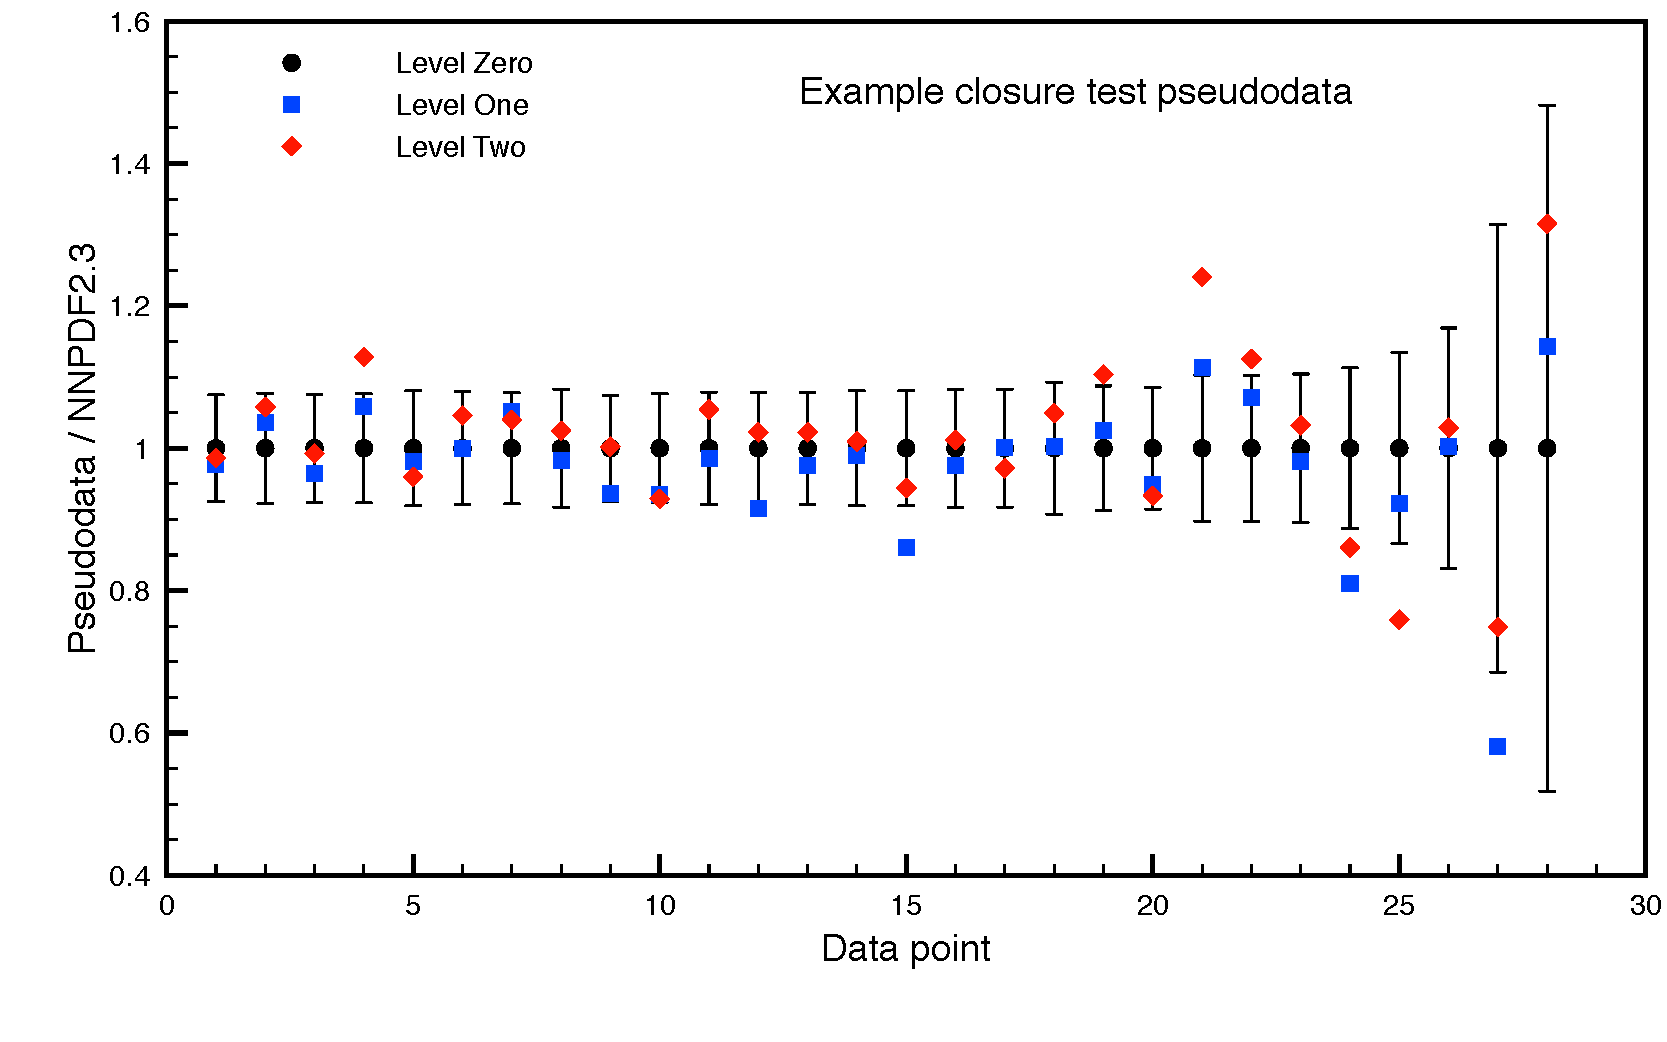
\includegraphics[width=0.9\textwidth]{7-PostLHC/figs/Closuretest_levels/closuretest_levels.pdf}
\caption[Closure test pseudodata example]{Examples of pseudodata used in a closure test for all three levels. The black circles show the level zero pseudodata, and the experimental error bars. The blue squares show the pseudodata after experimental noise has been simulated (level one) and the red diamonds after both statistical noise simulation and Monte Carlo replica generation (level two). All points are normalised to the generating PDF set (NNPDF2.3).}
\label{fig:closurepseudodata}
\end{figure}

The new structure present in the {\tt nnpdf++} code, particularly the modular treatment of experimental data and theoretical predictions, allows for the straightforward use of predictions in the place of experimental data while keeping the experimental covariance matrices intact. The closure testing method has therefore been extensively applied to the development of the NNPDF methodology, with the procedure used for the NNPDF3.0 determination being guided largely by results from closure testing. Here we shall outline some general results, before demonstrating the application of the procedure to methodological development in the subsequent sections.

\subsubsection{Early closure tests}
The earliest NNPDF closure tests were conducted to assess the usefulness of the procedure, and performed with the full NNPDF2.3 procedure. As an initial test, a fit was performed to the toy PDF parametrisation as used in the Les Houches evolution benchmarks~\cite{Giele:2002hx}, a parametrisation based upon the CTEQ5M determination~\cite{Lai:1999wy}. In this set, the initial state distributions are given as

\begin{eqnarray}
\label{gsav-eq9}
  xu_v(x,\mu_{\rm f,0}^2)       &\! =\! & 5.107200\: x^{0.8}\: (1-x)^3,  
    \nonumber \\
  xd_v(x,\mu_{\rm f,0}^2)       &\! =\! & 3.064320\: x^{0.8}\: (1-x)^4,  
    \nonumber \\
  xg\,(x,\mu_{\rm f,0}^2)       &\! =\! & 1.700000\, x^{-0.1} (1-x)^5, 
    \nonumber \\
  x\bar{d}\,(x,\mu_{\rm f,0}^2) &\! =\! & .1939875\, x^{-0.1} (1-x)^6,
    \nonumber\\
  x\bar{u}\,(x,\mu_{\rm f,0}^2) &\! =\! & (1-x)\: x\bar{d}\,(x,\mu_{\rm f,0}^2),
    \nonumber\\
  xs\,(x,\mu_{\rm f,0}^2)       &\! =\! & x\bar{s}\,(x,\mu_{\rm f,0}^2) 
    \: = \: 0.2\, x(\bar{u}+\bar{d}\,)(x,\mu_{\rm f,0}^2),
\end{eqnarray}
where $u_v$ and $d_v$ refer to the up and down valence distributions respectively. Predictions for the NNPDF2.3 dataset were made according to these distributions, and used in the place of experimental data. Experimental noise was simulated in the pseudodata by application of the same procedure used to provide artificial data replicas. The full NNPDF2.3 procedure including Monte Carlo artificial replicas was then applied to the dataset, the resulting PDF set therefore being a level two type closure test where the generating PDF set should be recovered by the fit within the estimated uncertainties.

\begin{figure}[ht]
\centering
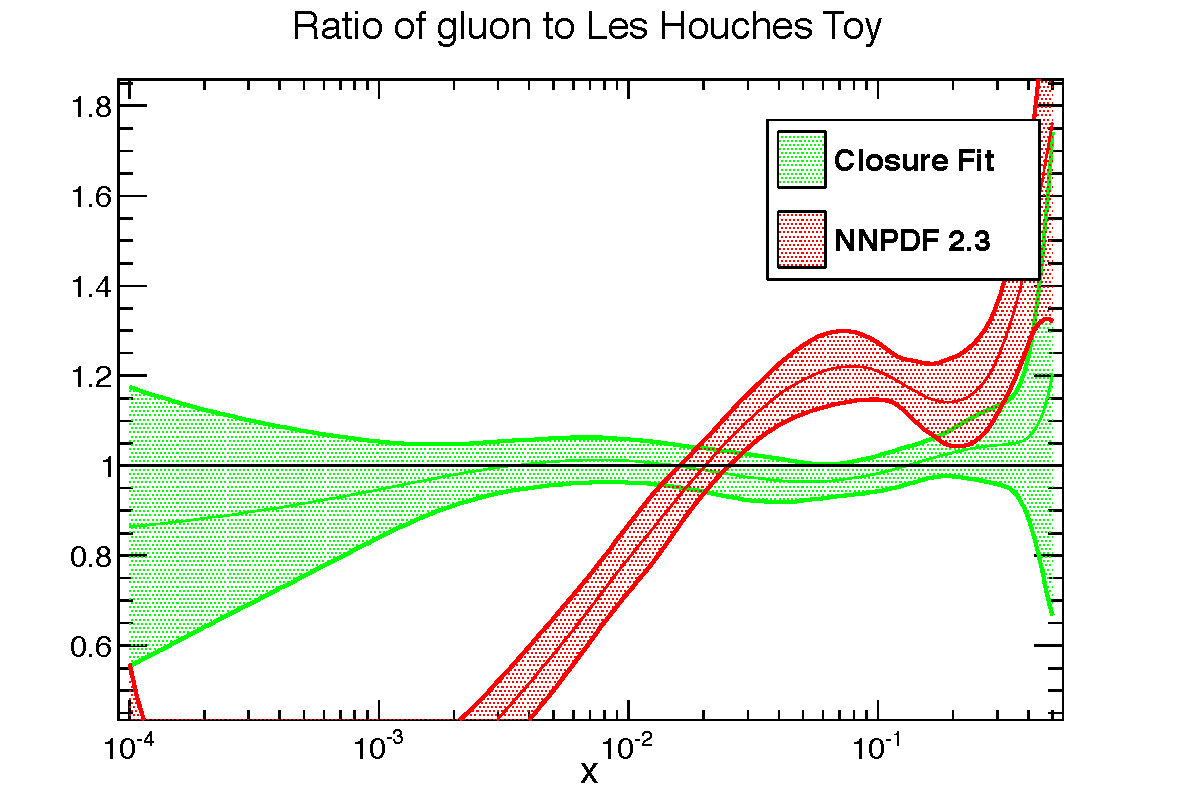
\includegraphics[width=0.48\textwidth]{7-PostLHC/figs/gluon.pdf}
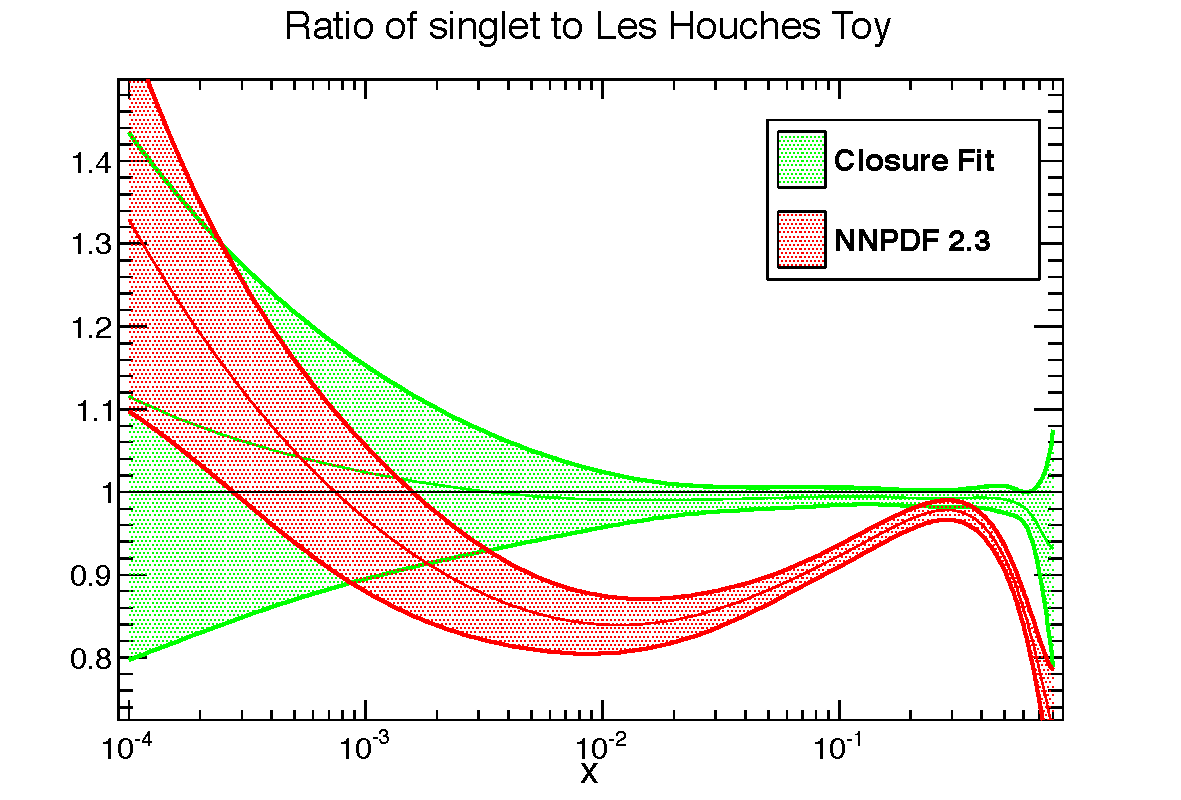
\includegraphics[width=0.48\textwidth]{7-PostLHC/figs/singlet.pdf}\\
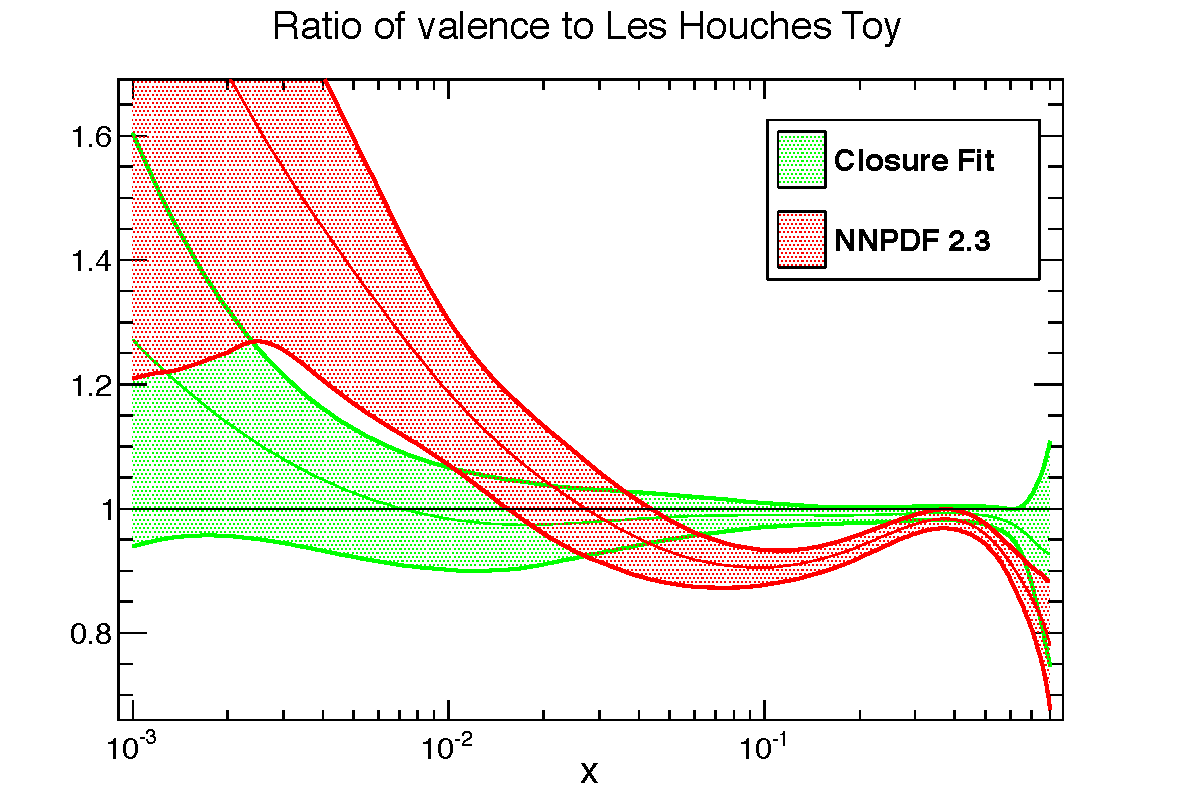
\includegraphics[width=0.48\textwidth]{7-PostLHC/figs/valence.pdf}
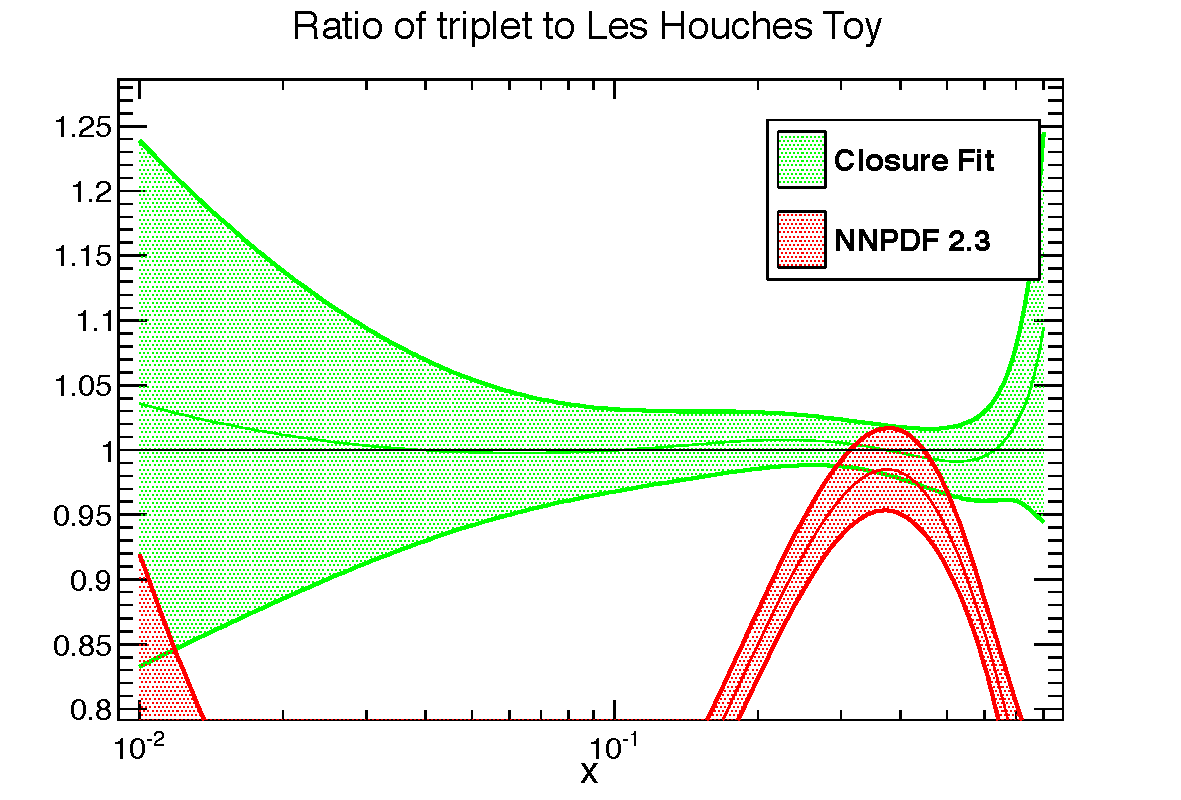
\includegraphics[width=0.48\textwidth]{7-PostLHC/figs/triplet.pdf}
\caption[PDFs obtained through a Closure test fit with toy PDFs as a generating function]{PDFs obtained through a closure test fit with Les Houches toy PDFs as a generating function, displayed as a ratio to the generating function. Shown are the distributions for the gluon, singlet, valence and triplet PDFs. In green are the results obtained through the closure test, and the red curves show the standard NNPDF2.3 result.}
\label{fig:LHtoyclosure1}
\end{figure}

Figure~\ref{fig:LHtoyclosure1} displays the results of the level two closure test fit with the Les Houches toy PDFs used as a generating function. The result demonstrates impressive agreement, with the NNPDF2.3 methodology able to accommodate the predictions of the Les Houches toy generating function despite it deviating significantly from the standard NNPDF2.3 result. For all four PDF combinations shown, the results of the closure test maintain distances of less than one standard deviation to the generating function across a wide kinematic range. Of additional interest are the strange distributions, relatively poorly constrainted by the data included in the pseudo-dataset. The strange valence in particular is set to zero in the Les Houches toy. Figure~\ref{fig:LHtoyclosure2} shows the results from the closure test for both the total strangeness and strange valence distributions, the NNPDF methodology is able to clearly reproduce the underlying law within uncertainties in both cases, and is able to comfortably resolve a zero strange valence contribution.

\begin{figure}[ht]
\centering
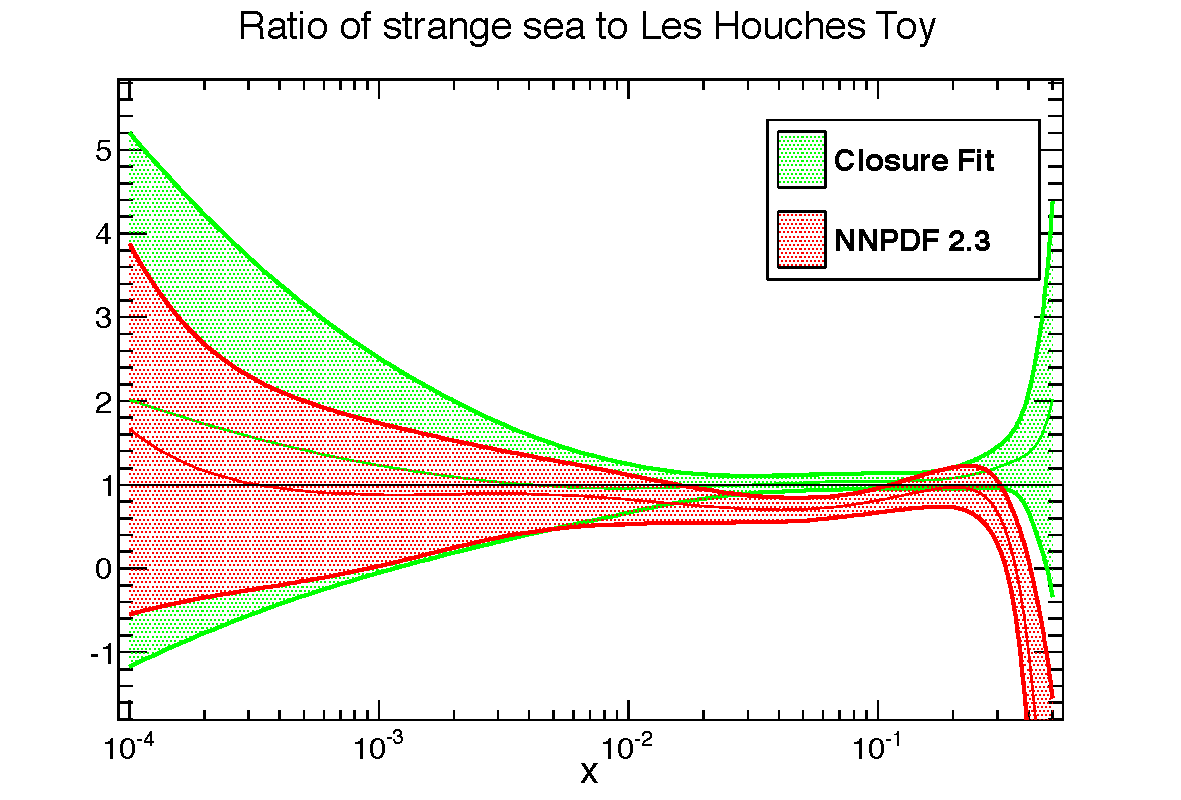
\includegraphics[width=0.48\textwidth]{7-PostLHC/figs/strangesea.pdf}
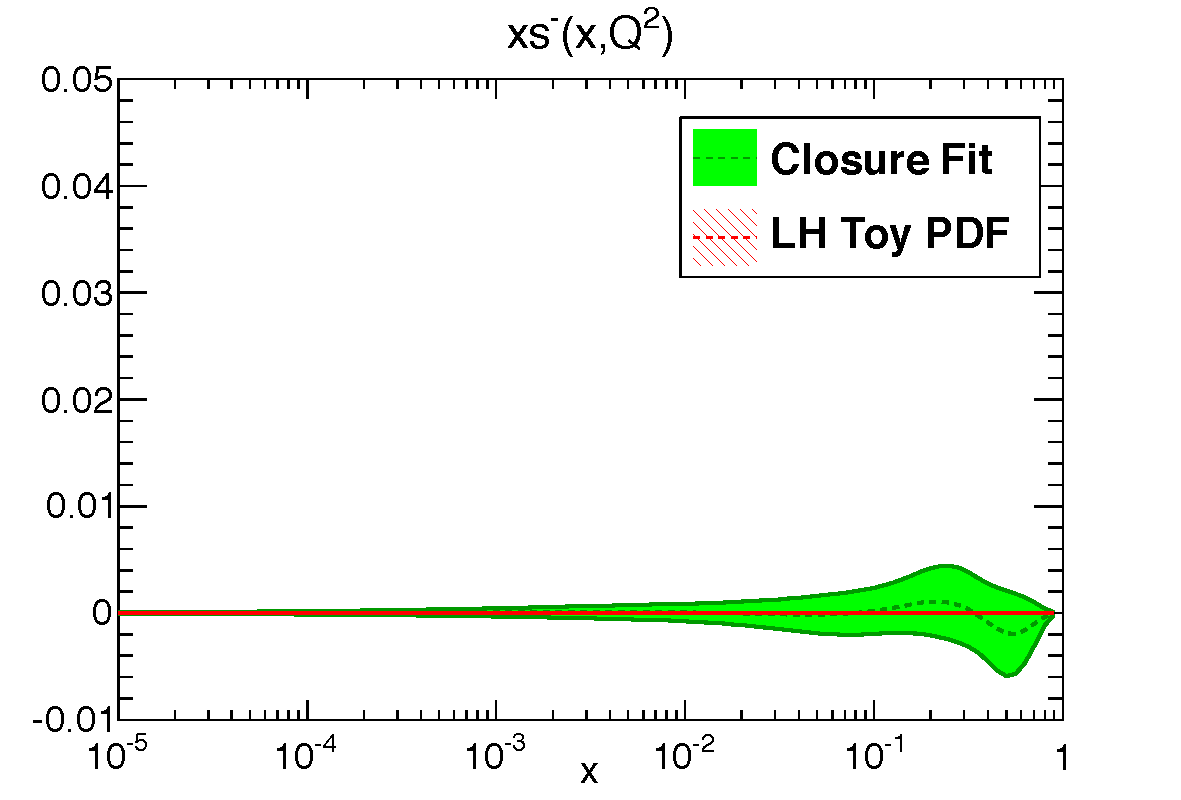
\includegraphics[width=0.48\textwidth]{7-PostLHC/figs/c1_n64.pdf}
\caption[Strange PDFs obtained through a Closure test fit with toy PDFs as a generating function]{Strange sea (left) and valence (right) PDFs obtained through a closure test fit with Les Houches toy PDFs as a generating function. The strange sea is presented as a ratio to the LH toy PDF, and the strange valence is presented directly as the PDF, with the (zero) LH toy line shown.}
\label{fig:LHtoyclosure2}
\end{figure}

The results are particularly impressive considering that this is a test of a methodology that has not been previously verified by closure test. The example case of a pseudo-dataset generated according to the Les Houches toy PDF is however a rather simplified case, and methodological refinements can be made by examining closure tests with greater structure in the generating function.

A good level of agreement can also be found at the level of the $\chi^2$ to both the pseudodata sample, and the real experimental data. In Figure~\ref{fig:CPPclosurechi2} we compare the fit quality of a closure test and its generating PDF dataset by dataset by presenting the $\chi^2$ to each measurement from both the closure test result and the generating PDF. In this case the generating function has considerably greater complexity, being an early {\tt nnpdf++} test fit with most of the NNPDF methodology in place. While agreement is generally very good, especially on the level of total $\chi^2$; we begin to see some elements of discrepancy in datasets sensitive to flavour separation and strangeness such as the NuTeV dataset and electroweak vector boson production data. Such discrepancies can help in pinpointing areas where further development is needed.


\begin{figure}[!]
\centering
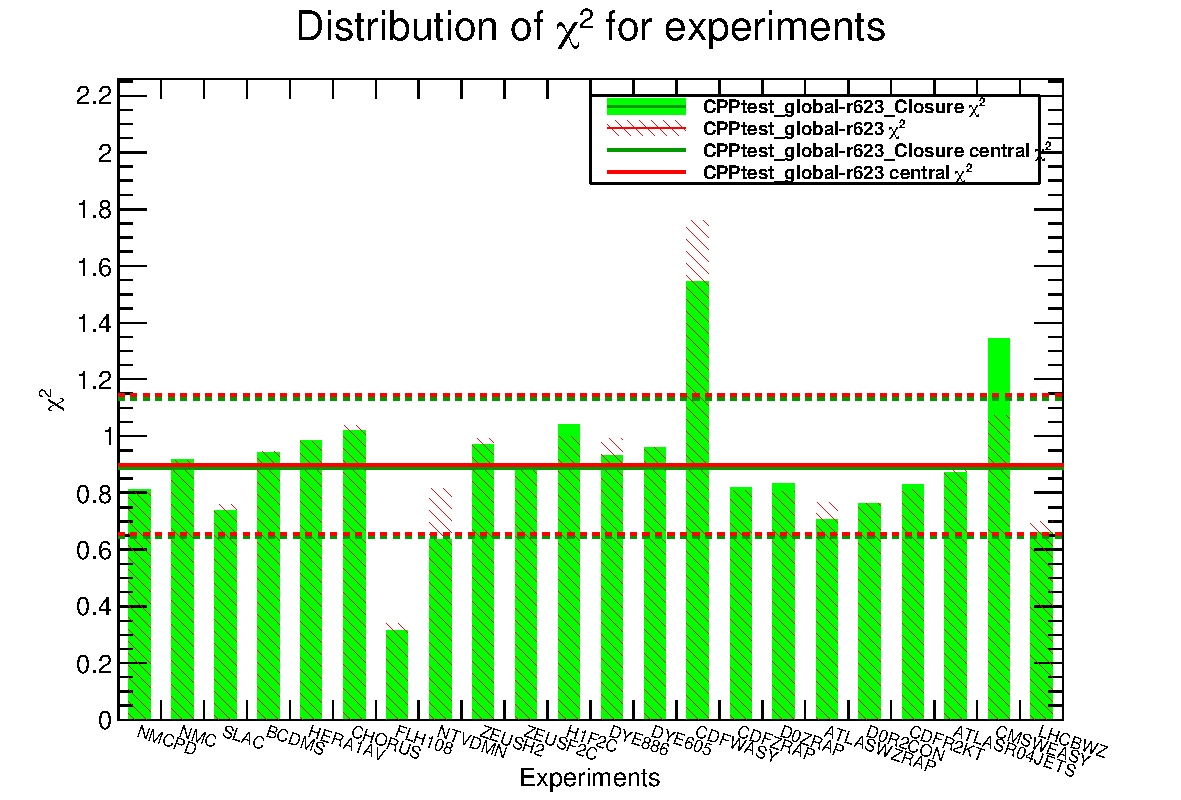
\includegraphics[width=0.48\textwidth]{7-PostLHC/figs/chi2_histo_nnpdf1.pdf}
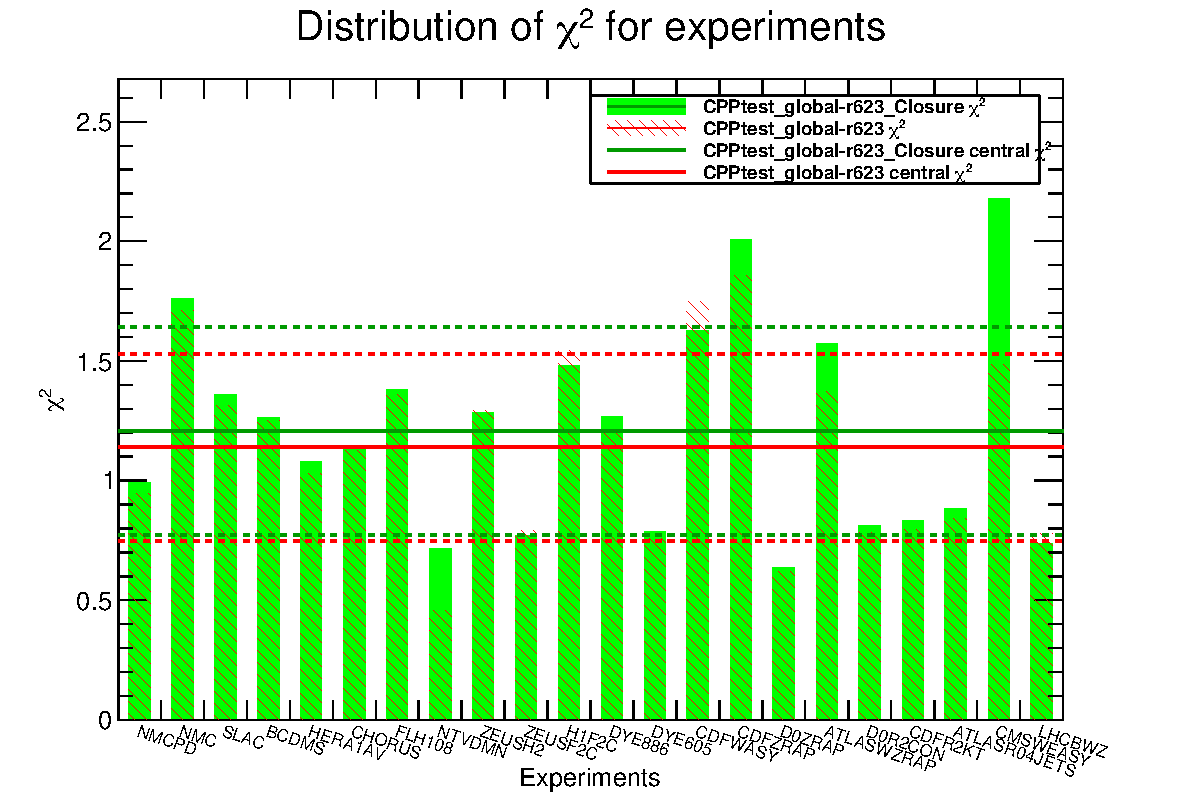
\includegraphics[width=0.48\textwidth]{7-PostLHC/figs/chi2_histo_nnpdf2.pdf}
\caption[$\chi^2$ values to the pseudo- and experimental-datasets of a closure fit and the generating PDF]{Example $\chi^2$ values to the pseudo- (left) and experimental- (right) datasets of a closure fit and the generating PDF from early {\tt nnpdf++} test fits. The red bars show the fit quality of the generating PDF set while the green bars demonstrate the $\chi^2$ for the closure test set. The horizontal lines indicate the average and $1\sigma$ of the fit qualities in their associated colours.}
\label{fig:CPPclosurechi2}
\end{figure}

\section{Preprocessing}

Early closure tests performed with the NNPDF2.3 methodology showed generally very good agreement between the produced PDFs and the underlying functions used to generate the pseudo-dataset. However some PDF combinations demonstrated rather poorer agreement than others, particularly distributions sensitive to flavour separation. Such disagreements became more apparent when considering closure tests to underlying functions with more structure than available in the Les Houches toy set. The disagreements were found to originate in the choice of the preprocessing exponents used in the definition of the NNPDF parametrisation. Recalling Eqn.~\ref{eq:NNPDF23param}, the structure of the basic NNPDF parametrisation follows
\be f(x) \propto x^{-\alpha} (1-x)^{\beta} \text{NN}(x),\ee
where NN represents the neural network itself, and $\alpha$ and $\beta$ are the preprocessing exponents randomised on a replica-by-replica basis at the start of a fit. The range in which the exponents were randomised has been fixed in the fits up to and including NNPDF2.3, set to a span large enough such that the dependence of the results upon the choice of range was minimised. In such a way the preprocessing was considered to provide a backbone for the neural-network fit and, aside from improving fitting efficiency, to have a minimal impact upon the results.

To study the effect of different preprocessing ranges we can look at estimators for the \emph{effective} asymptotic exponents,
\be \alpha_{\text{eff}} = -\frac{\log{(|f(x)|)}}{\log(x)},\quad\quad \beta_{\text{eff}} = \frac{\log{(|f(x)|)}}{\log(1-x)}, \ee
such that in the limits of $x\to0,1$ the exponents $\alpha,\beta$ are recovered. By examining these effective exponents in the high- and low-$x$ regions, we can ascertain if there is a data preference for a different preprocessing range than was used in a fit, and if the preprocessing range used was too restrictive.

In Figure~\ref{fig:preproc1} an example preprocessing analysis is shown for a closure test based upon an MSTW08 underlying law at NLO. The sea asymmetry $\bar{u} -\bar{d}$ is shown for two choices of preprocessing range, the NNPDF2.3 standard and a range modified to better accommodate the data preference visible in the effective exponents. From the figure we can see that the choice of exponent randomisation range has a significant effect on the resulting distributions, and that the effective exponents can show a clear data preference for a different range. In Figure~\ref{fig:preproc2} we can see the same analysis applied to the triplet PDF where similar conclusions may be drawn.

These analyses demonstrate that the sensitivity to the preprocessing exponent randomisation ranges is somewhat larger than suspected previously, and needs to be studied in detail in order to avoid minimisation difficulties in a fit where the preprocessing ranges are ill-suited to the dataset. Furthermore, the uncertainty bulges visible in both the triplet and sea asymmetry distributions in Figures~\ref{fig:preproc1} and~\ref{fig:preproc2} are generated by the preprocessing suppressing genuine data uncertainty in the asymptotic regions. These problems may be alleviated by lifting the requirement that such distributions should be preprocessed to zero at low-$x$, and implementing a procedure for the iterative and data-driven determination of preprocessing exponents.

To improve the minimisation performance, hampered by ill-suited preprocessing, NNPDF fits have now adopted the following iterative procedure for the determination of both high and low-$x$ randomisation ranges:

\begin{itemize}
\item \textbf{Singlet and gluon PDFs}\\
Exponent randomisation ranges are set to be twice the $1\sigma$ interval of the previous iteration's effective exponents
at the asymptotic points.
\clearpage
\item \textbf{Nonsinglet PDF combinations}\\
The low-$x$ randomisation interval is set to be the maximal extent of two effective exponent ranges; twice the $1\sigma$ interval at the asymptotic point and twice the $1\sigma$ interval at the point $x=1\times 10^{-3}$. The high-$x$ interval is set identically as with the singlet and gluon.
\end{itemize} 

In such a way convergence of the randomisation interval can be established typically in two or three fit iterations, and the preprocessing exponents are obtained from the preference of the experimental dataset. As an example of a fit generated from such an iterative procedure consider Figure~\ref{fig:preproc3} which demonstrates the preprocessing analysis for the $\Delta_s$ and Triplet distributions resulting from the new procedure. In comparison to Figure~\ref{fig:preproc1} where the old settings are used, the low-$x$ preprocessing ranges have relaxed considerably and are no longer constrained by the chosen exponent range but driven by the experimental data. Furthermore the agreement with the underlying law is noticeably improved over the previous result shown in Figure~\ref{fig:preproc1}. 

\begin{figure}[hp!]
\centering
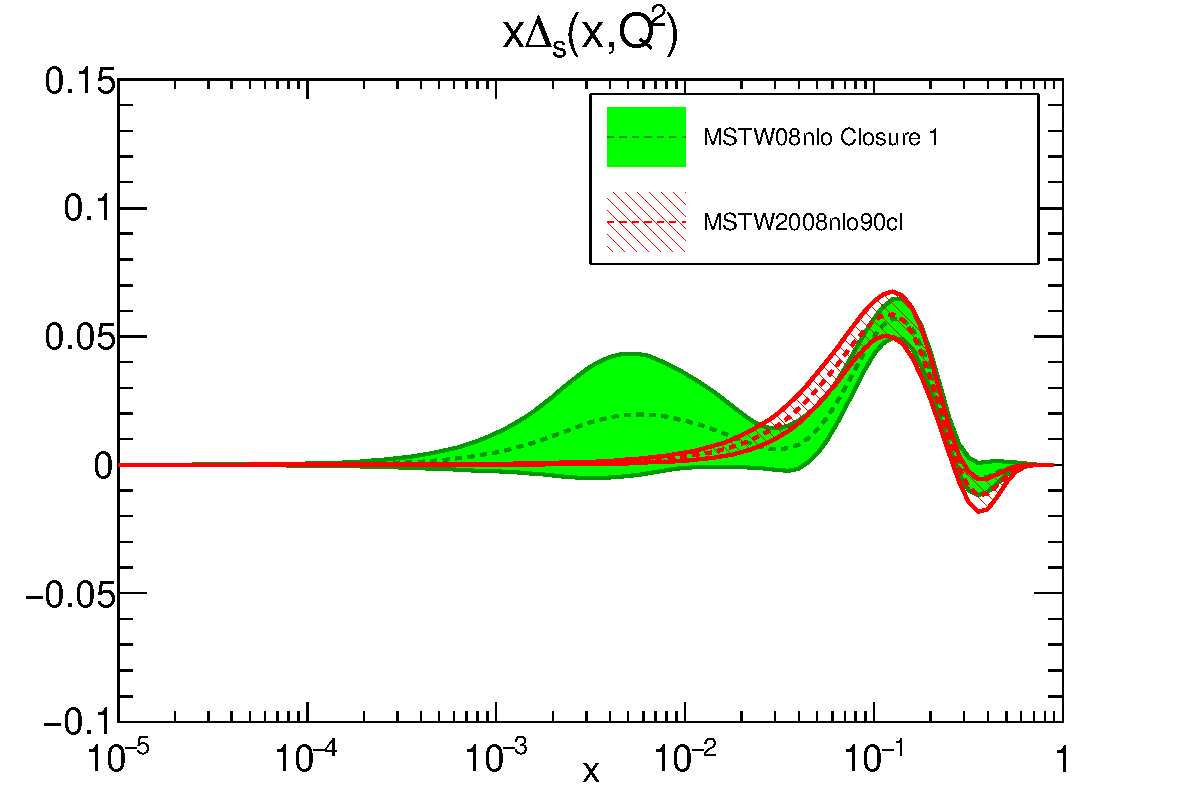
\includegraphics[width=0.48\textwidth]{7-PostLHC/figs/Preproc1/pdf_xDs_log_others.pdf}
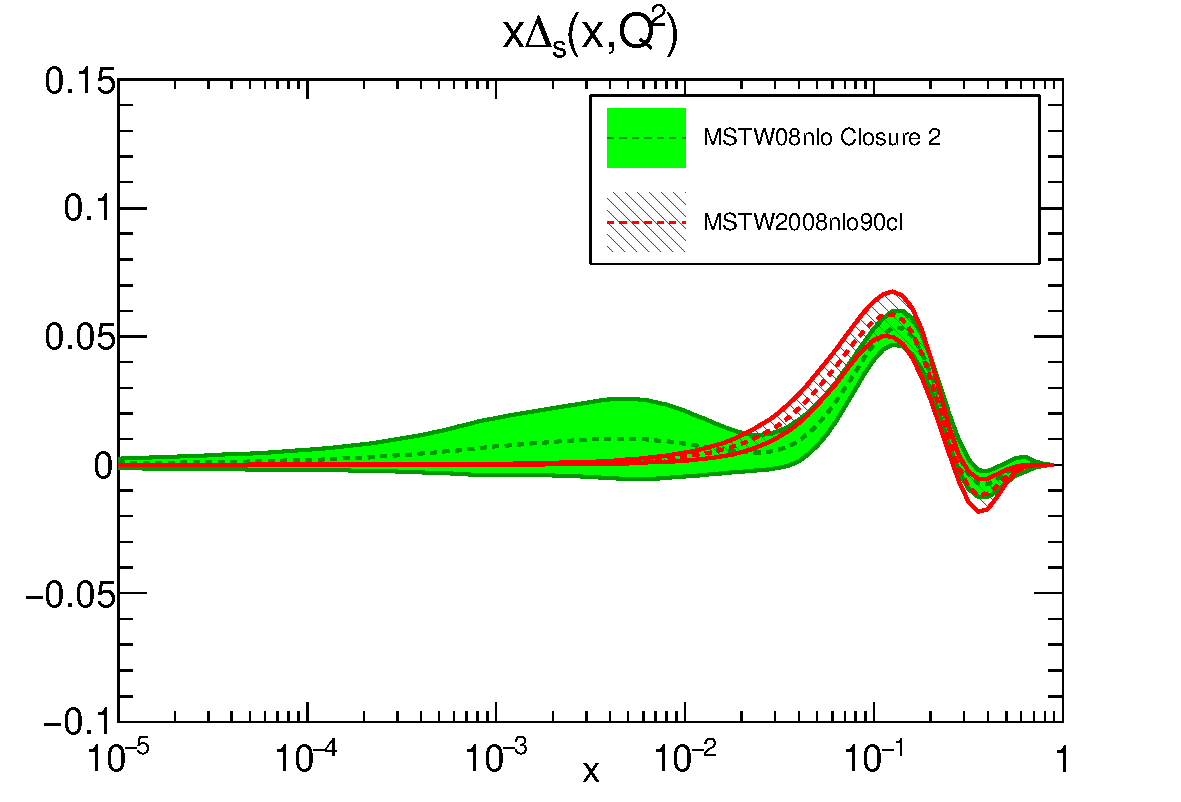
\includegraphics[width=0.48\textwidth]{7-PostLHC/figs/Preproc2/pdf_xDs_log_others.pdf}
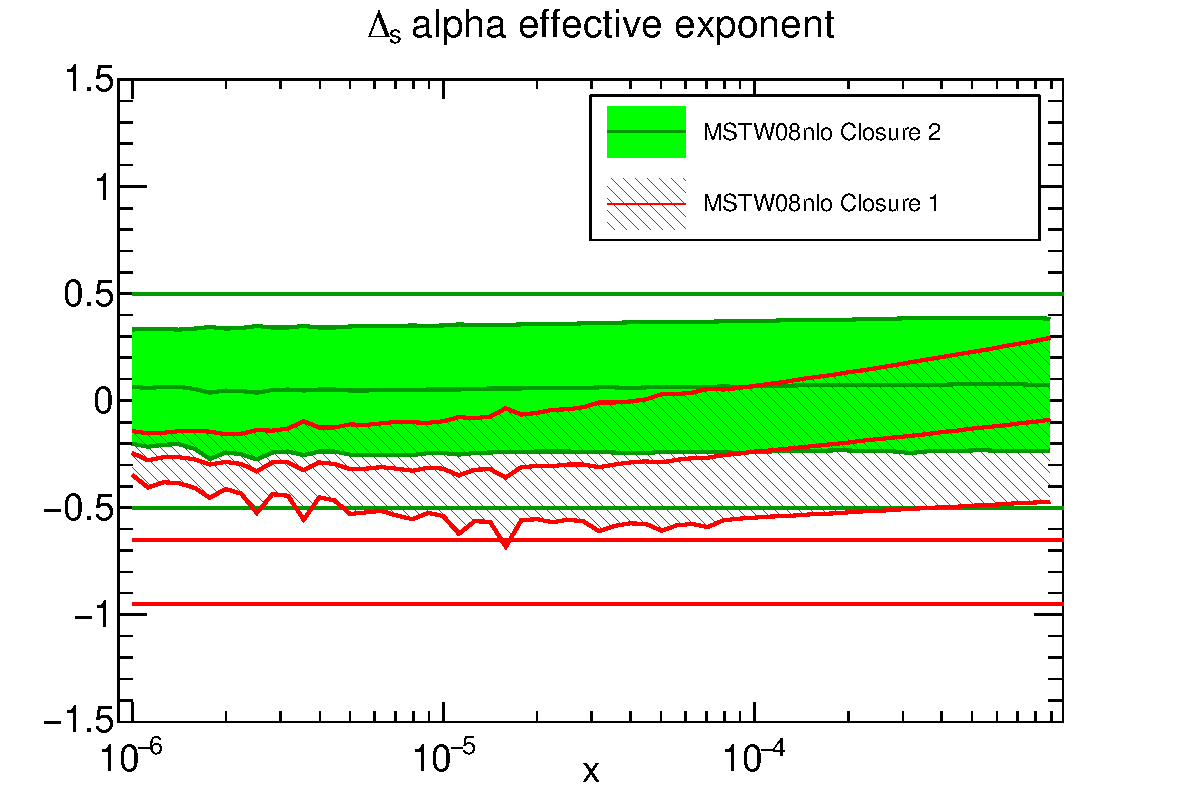
\includegraphics[width=0.48\textwidth]{7-PostLHC/figs/Preproc2/alphapreproc_4.pdf}
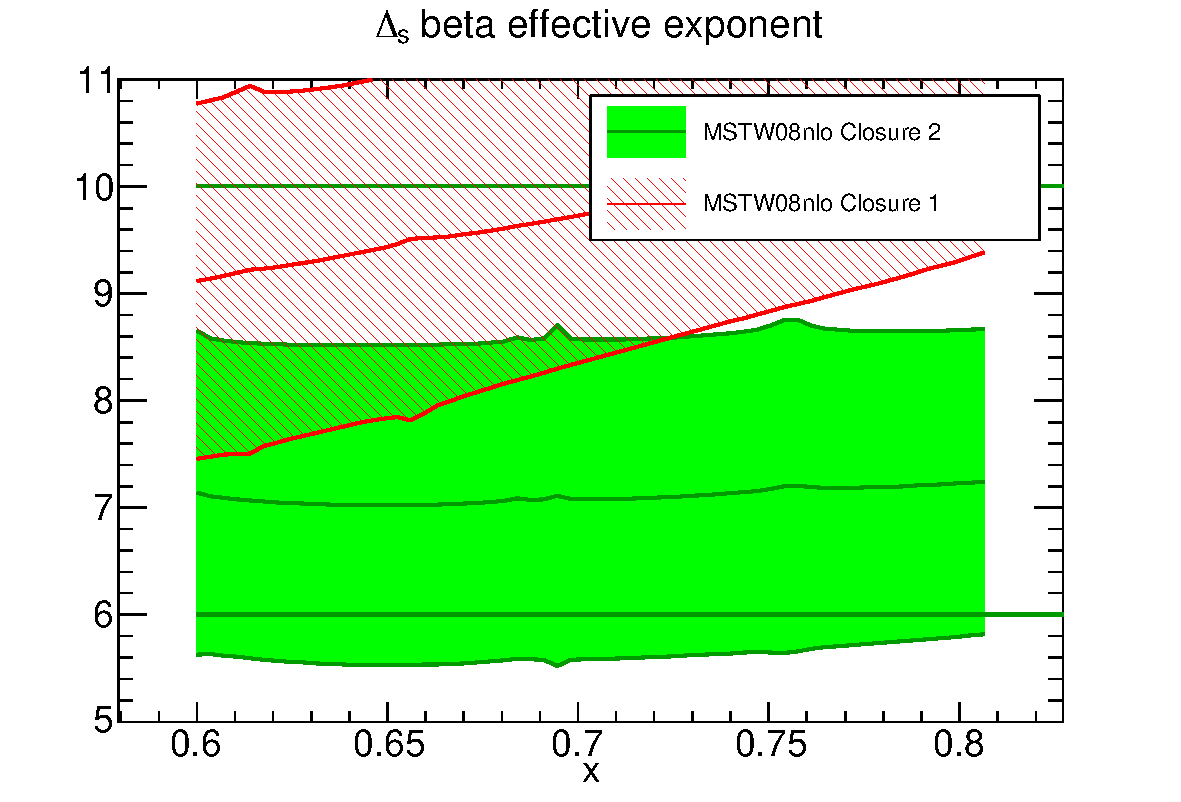
\includegraphics[width=0.48\textwidth]{7-PostLHC/figs/Preproc2/betapreproc_4.pdf}
\caption[Demonstration of the impact made by changes in preprocessing to the sea asymmetry PDF in a closure test fit]{Demonstration of the impact made by changes in preprocessing to the sea asymmetry PDF in a closure test fit to an MSTW08 NLO underlying law. The top two figures demonstrate the results for the $\Delta_s$ distribution for two choices of preprocessing ranges, with the left figure using NNPDF2.3 standard preprocessing. In both cases, the red curve shows the underlying law used in the Closure test. The right figure demonstrates slightly improved agreement, particularly at low-$x$. The lower figures show the low and high $x$ effective exponent plots for the two ranges. The solid horizontal lines delineate the regions in which the preprocessing exponents were initialised, and the bands show the $1\sigma$ contours of the effective exponents.}
\label{fig:preproc1}
\end{figure}

\clearpage
\begin{figure}[!]
\centering
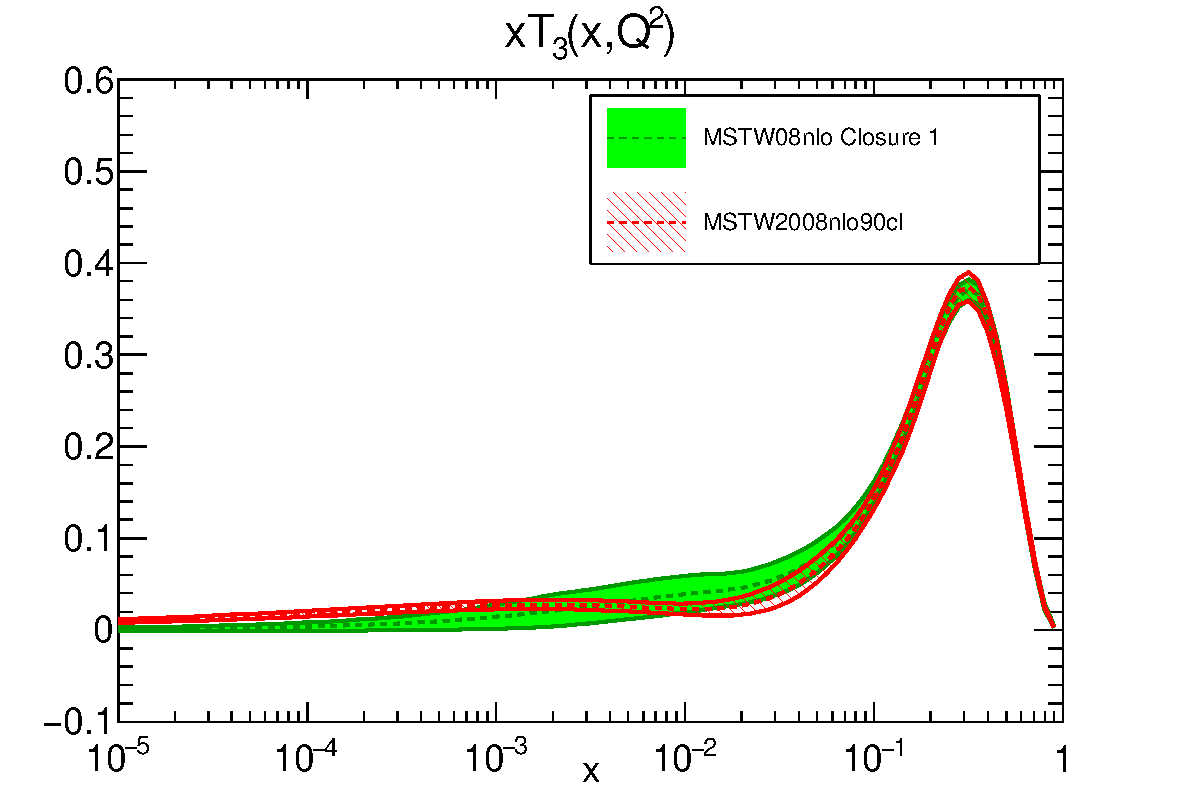
\includegraphics[width=0.42\textwidth]{7-PostLHC/figs/Preproc1/pdf_xT3_log_others.pdf}
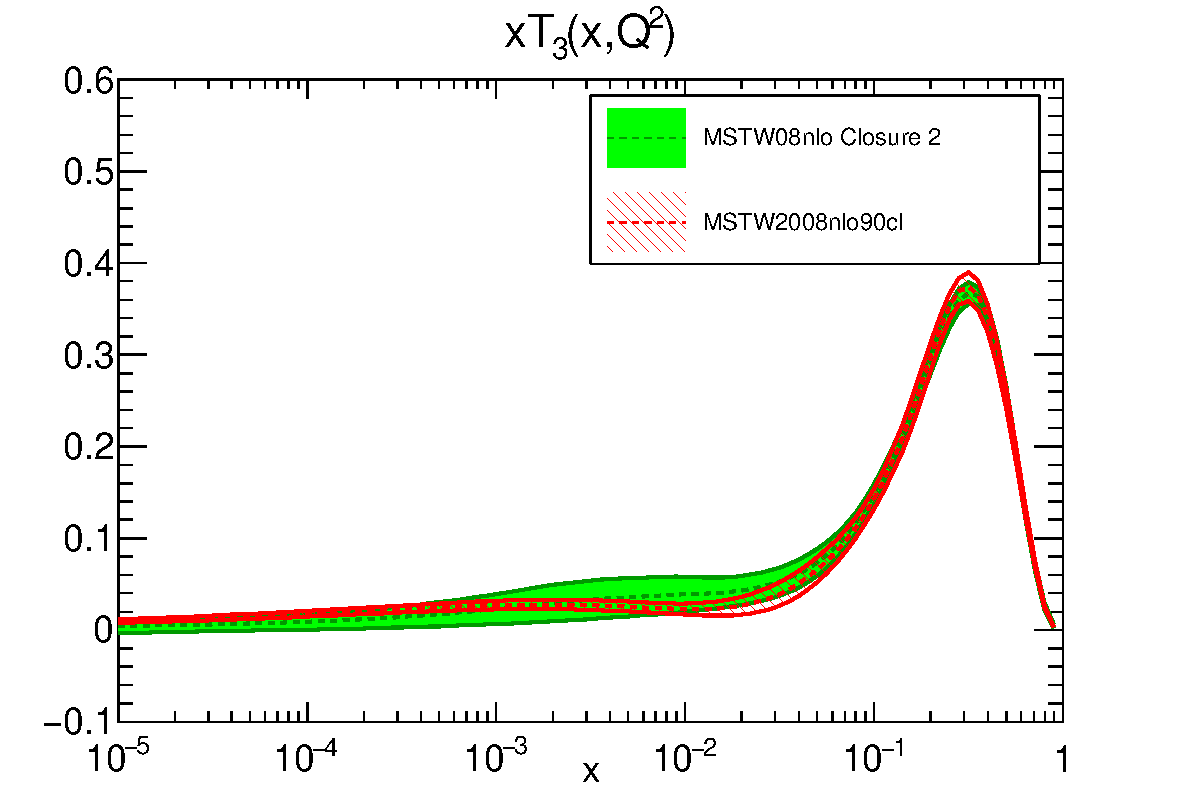
\includegraphics[width=0.42\textwidth]{7-PostLHC/figs/Preproc2/pdf_xT3_log_others.pdf}
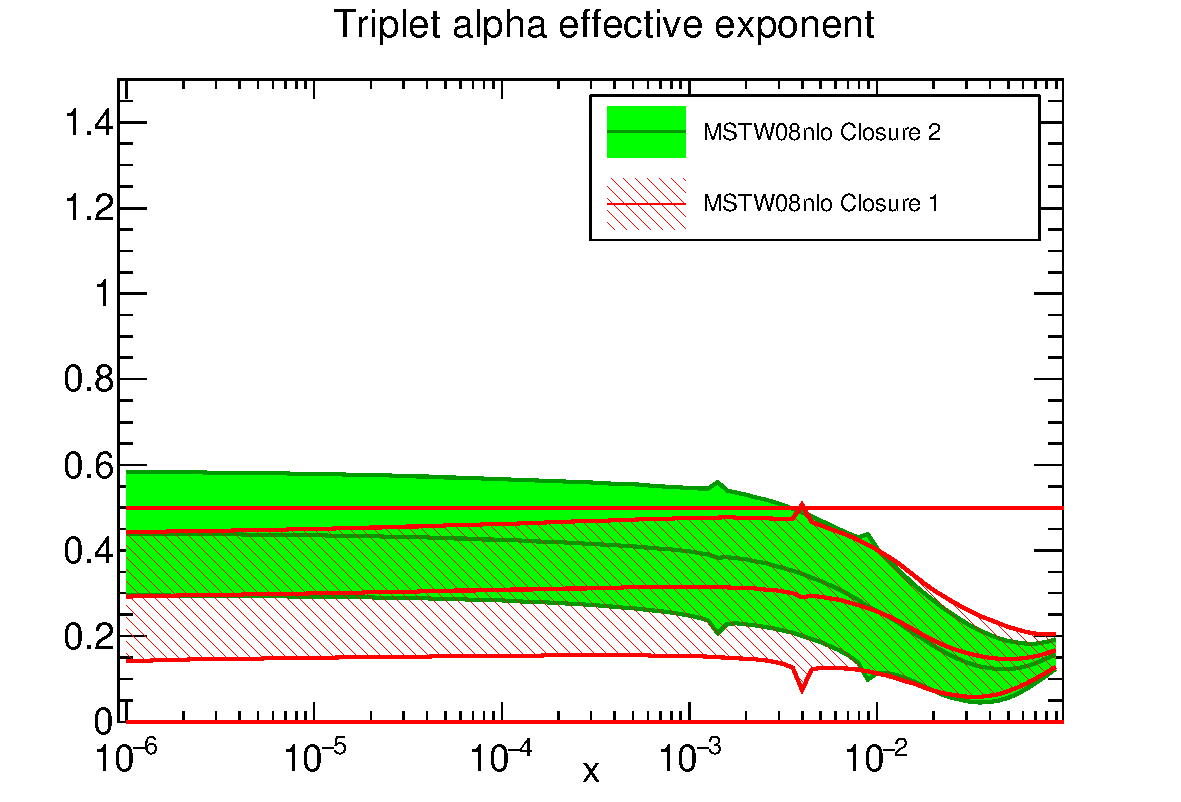
\includegraphics[width=0.42\textwidth]{7-PostLHC/figs/Preproc2/alphapreproc_3.pdf}
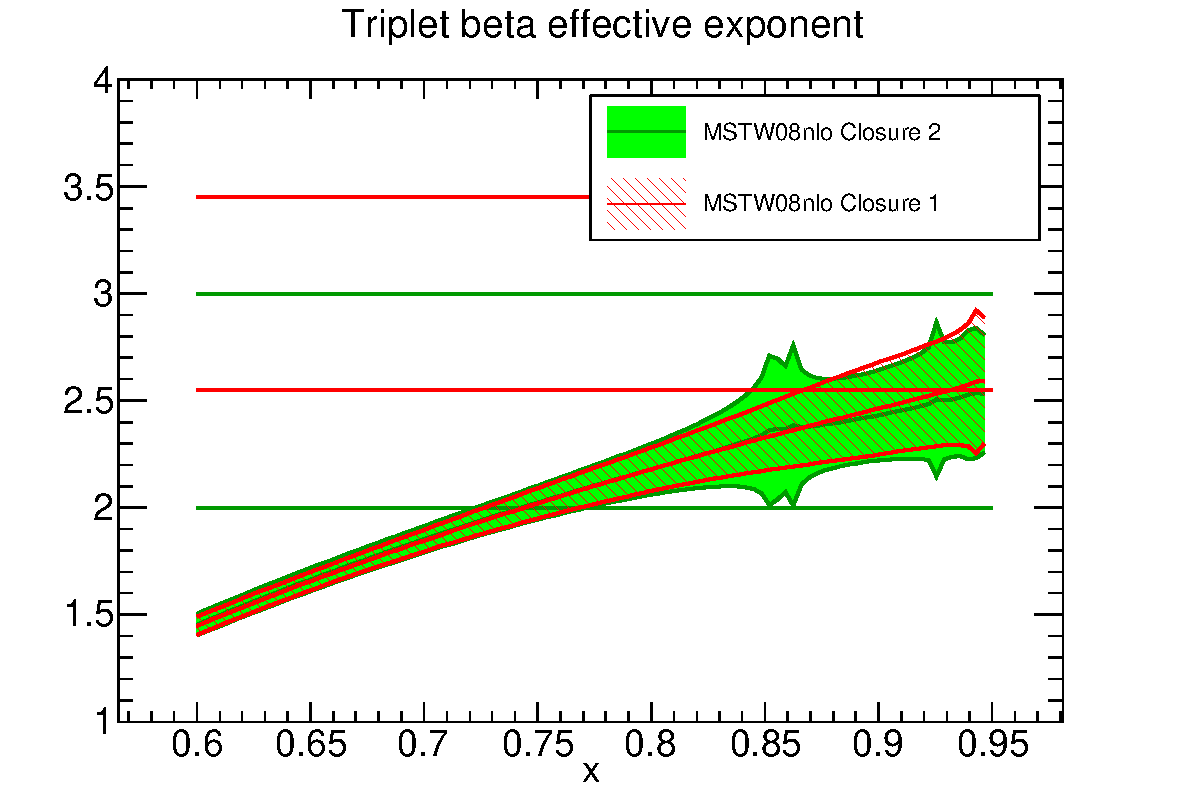
\includegraphics[width=0.42\textwidth]{7-PostLHC/figs/Preproc2/betapreproc_3.pdf}
\caption[Demonstration of the impact made by changes in preprocessing to the triplet PDF in a closure test fit]{A further preprocessing analysis as in Figure~\ref{fig:preproc1}, performed upon the Triplet PDF combination for the same two closure test fits.}
\label{fig:preproc2}
\end{figure}

\begin{figure}[!]
\centering
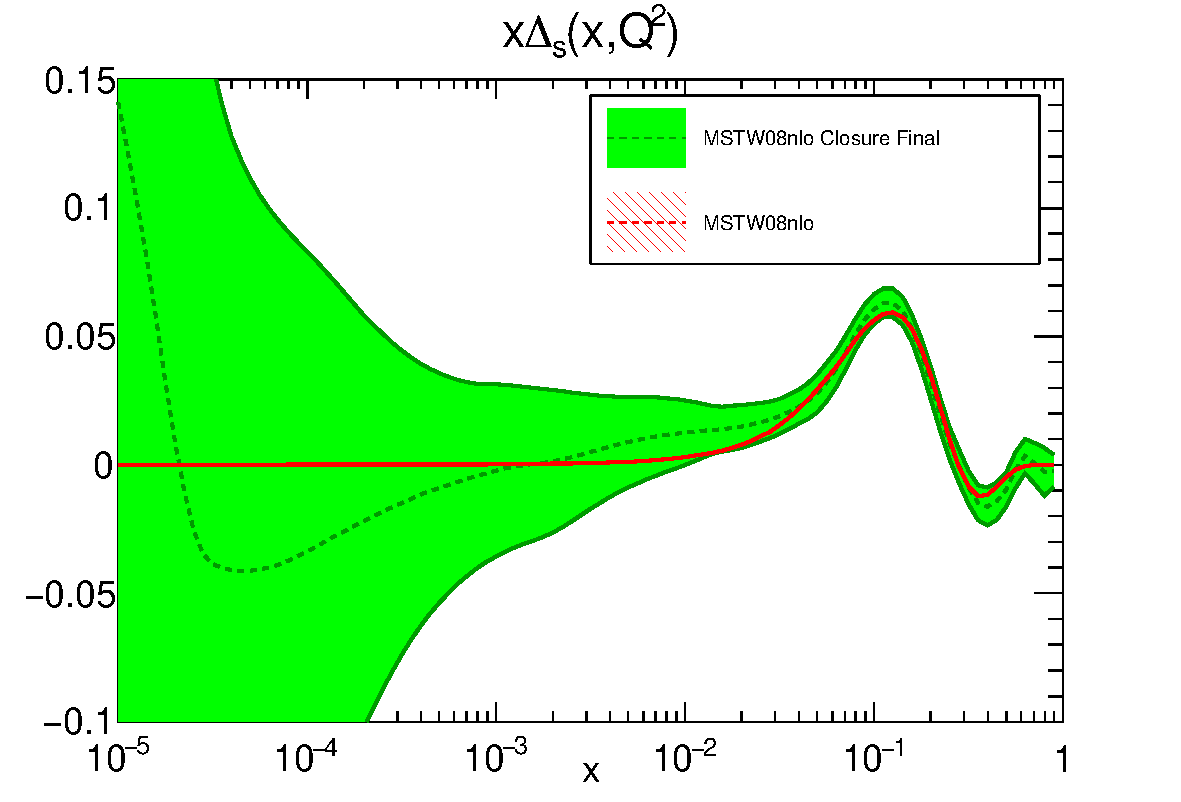
\includegraphics[width=0.42\textwidth]{7-PostLHC/figs/PreprocFixed/pdf_xDs_log_others.pdf}
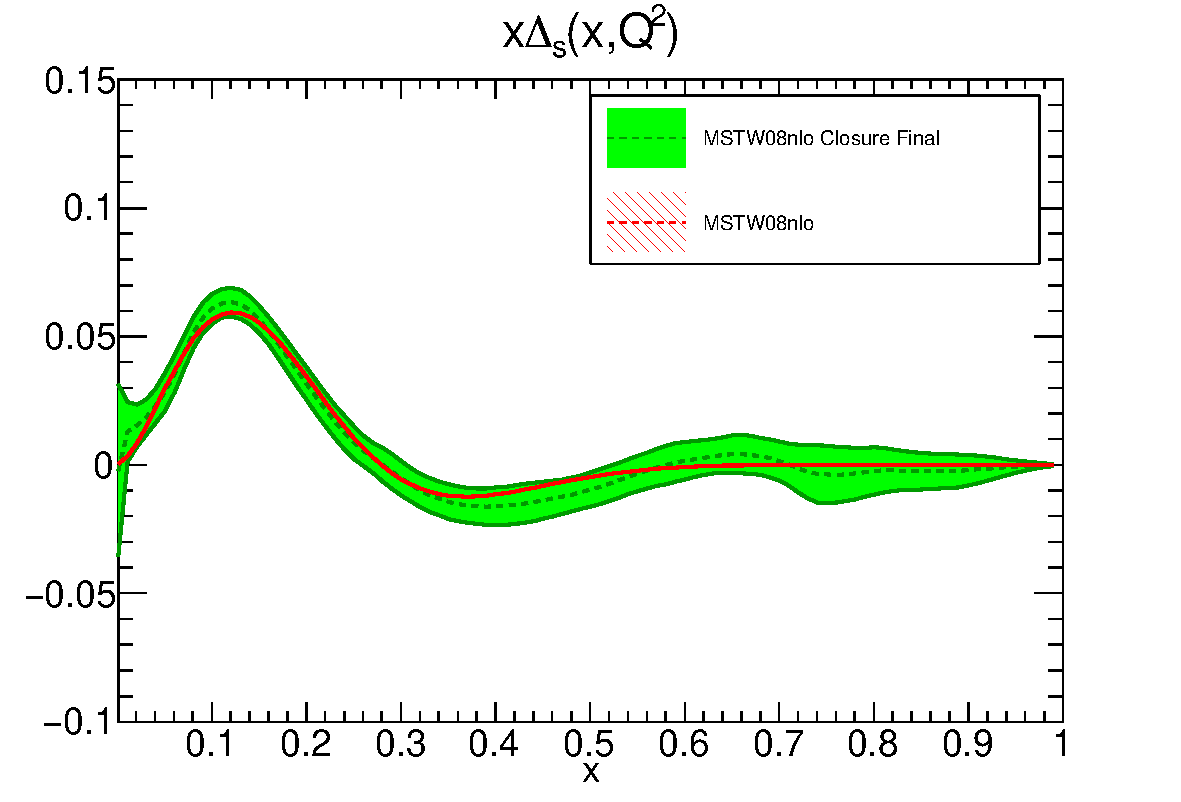
\includegraphics[width=0.42\textwidth]{7-PostLHC/figs/PreprocFixed/pdf_xDs_others.pdf}
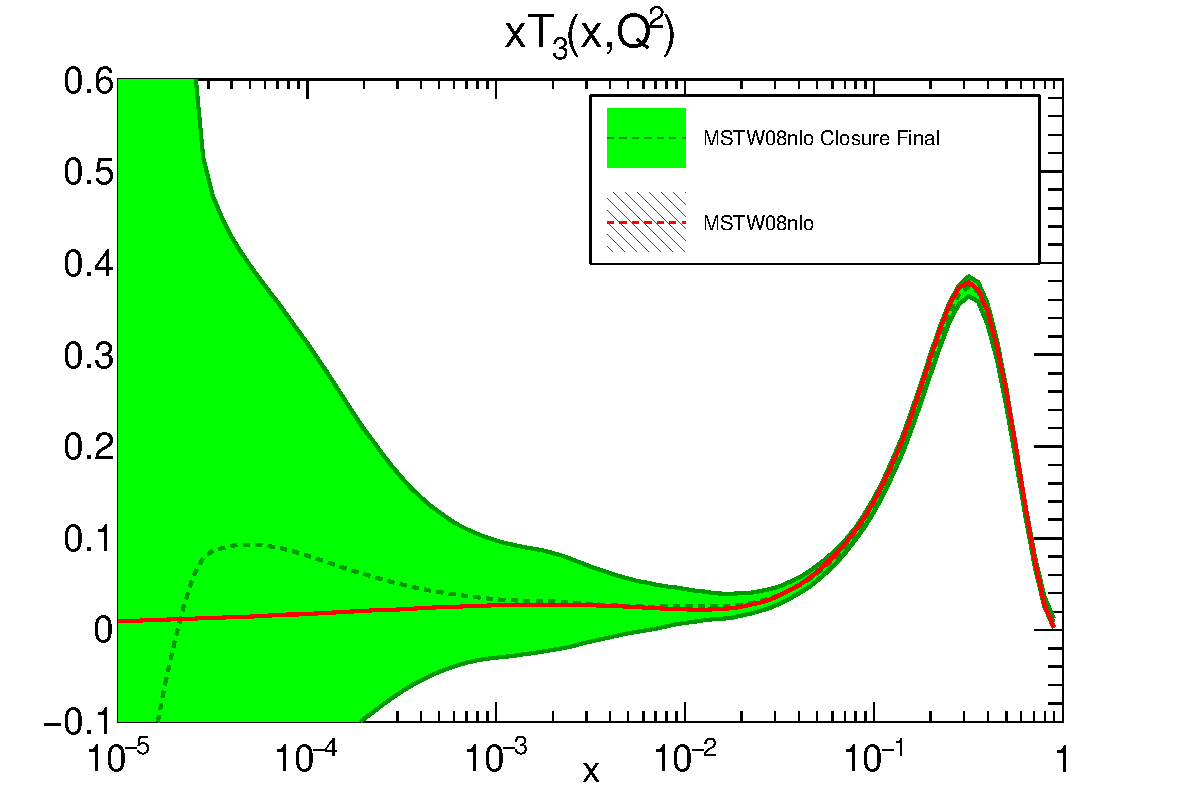
\includegraphics[width=0.42\textwidth]{7-PostLHC/figs/PreprocFixed/pdf_xT3_log_others.pdf}
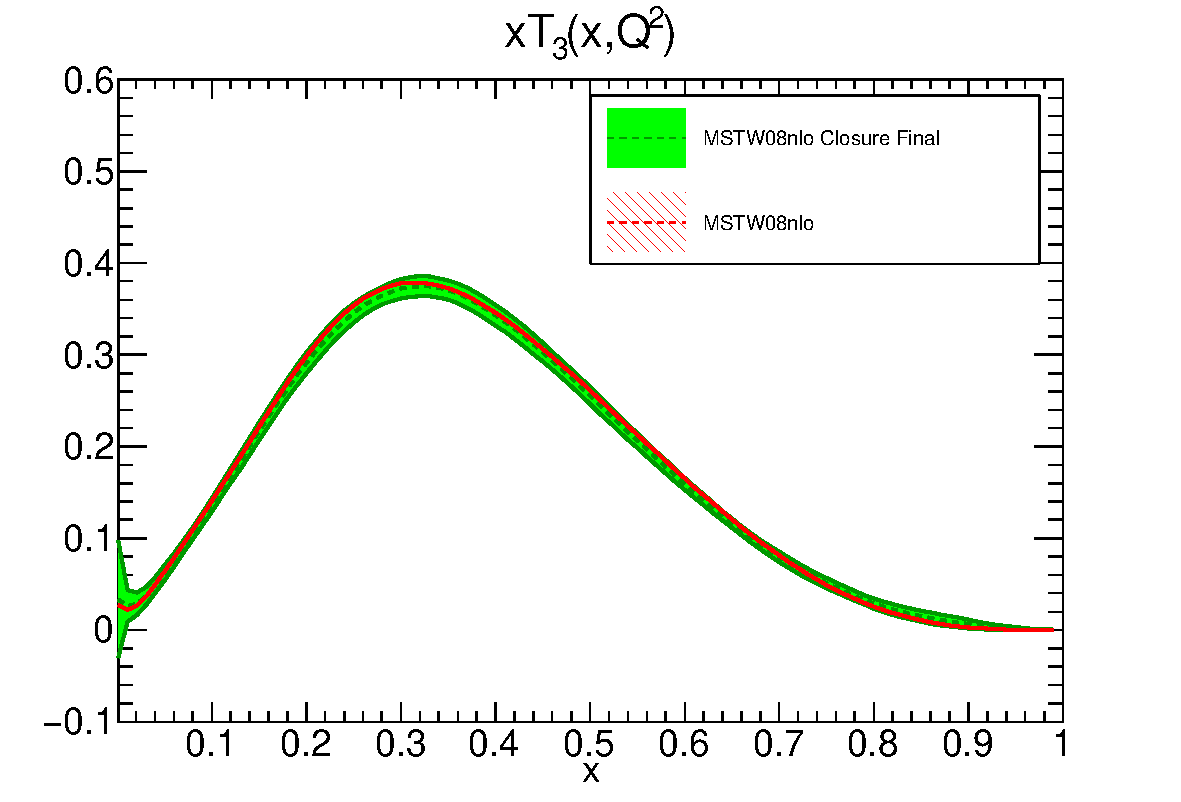
\includegraphics[width=0.42\textwidth]{7-PostLHC/figs/PreprocFixed/pdf_xT3_others.pdf}
\caption[Impact of improved preprocessing range selection in the sea asymmetry and triplet PDFs]{Impact of improved preprocessing range selection in the sea asymmetry and triplet PDFs. The top figures demonstrate the $\Delta_s$ PDF obtained via a closure test to MSTW08 using the improved preprocessing procedure in green, with the underlying law shown in red. The figures below show the equivalent plots for the triplet PDF with the improved preprocessing ranges.}
\label{fig:preproc3}
\end{figure}
\clearpage

% Old figures
%\begin{figure}[!]
%\centering
%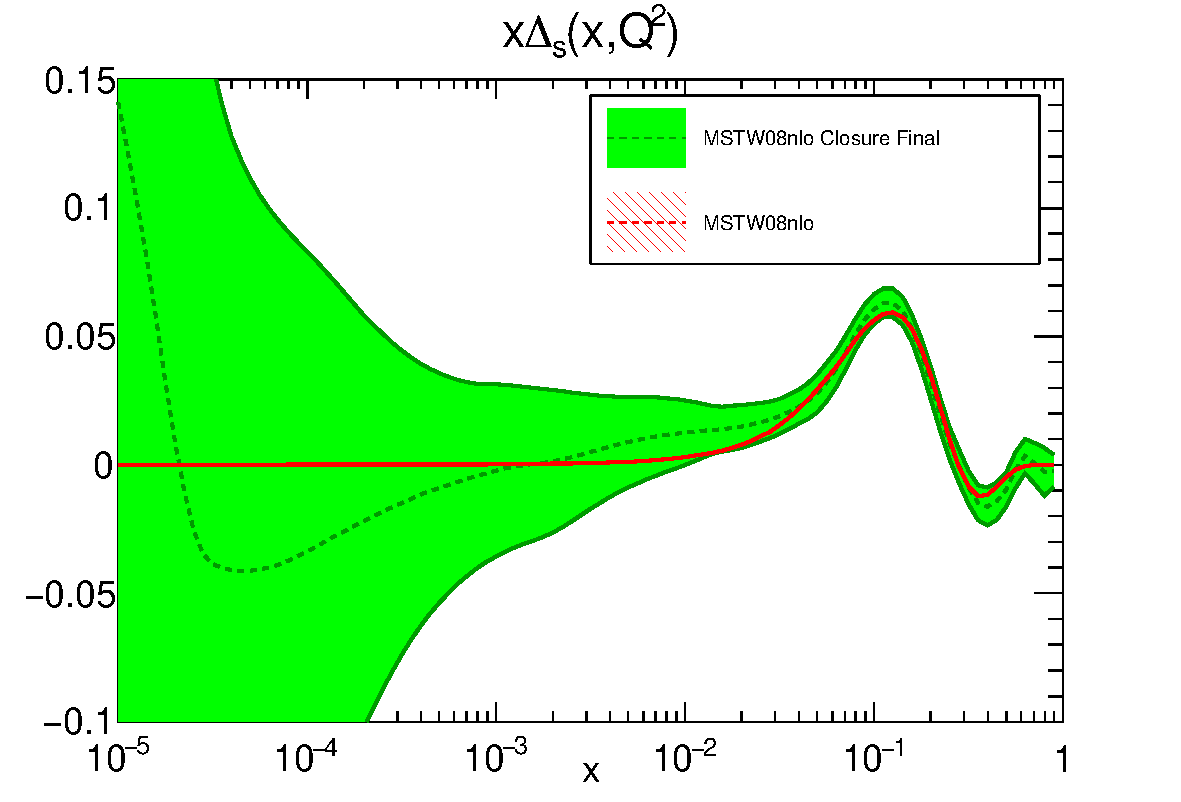
\includegraphics[width=0.42\textwidth]{7-PostLHC/figs/PreprocFixed/pdf_xDs_log_others.pdf}
%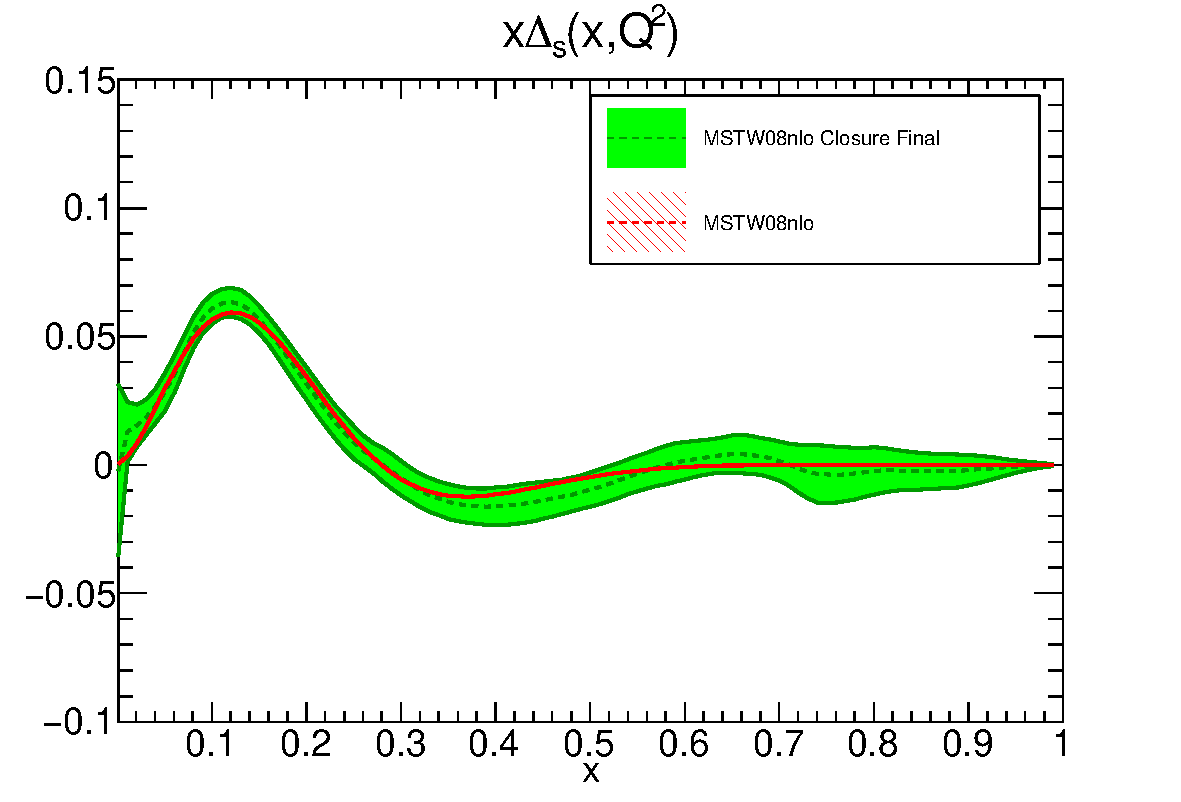
\includegraphics[width=0.42\textwidth]{7-PostLHC/figs/PreprocFixed/pdf_xDs_others.pdf}
%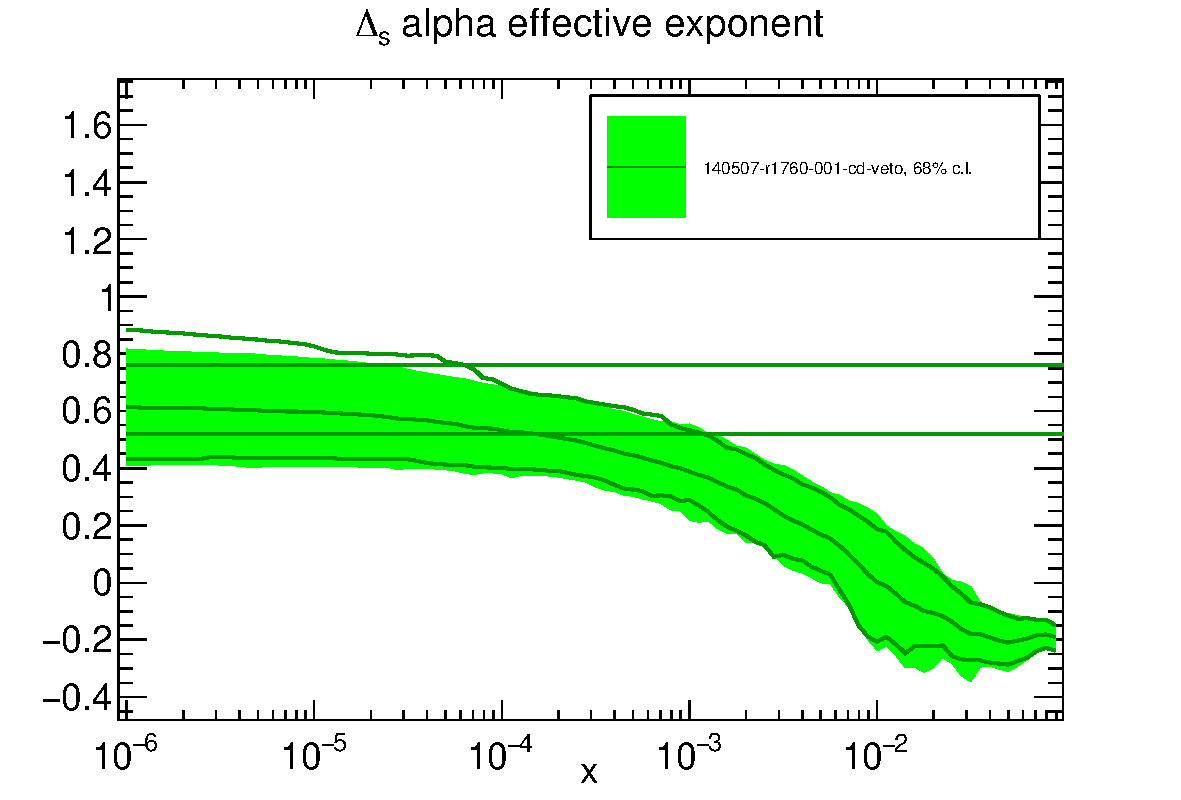
\includegraphics[width=0.42\textwidth]{7-PostLHC/figs/PreprocFixed/alphapreproc_4.pdf}
%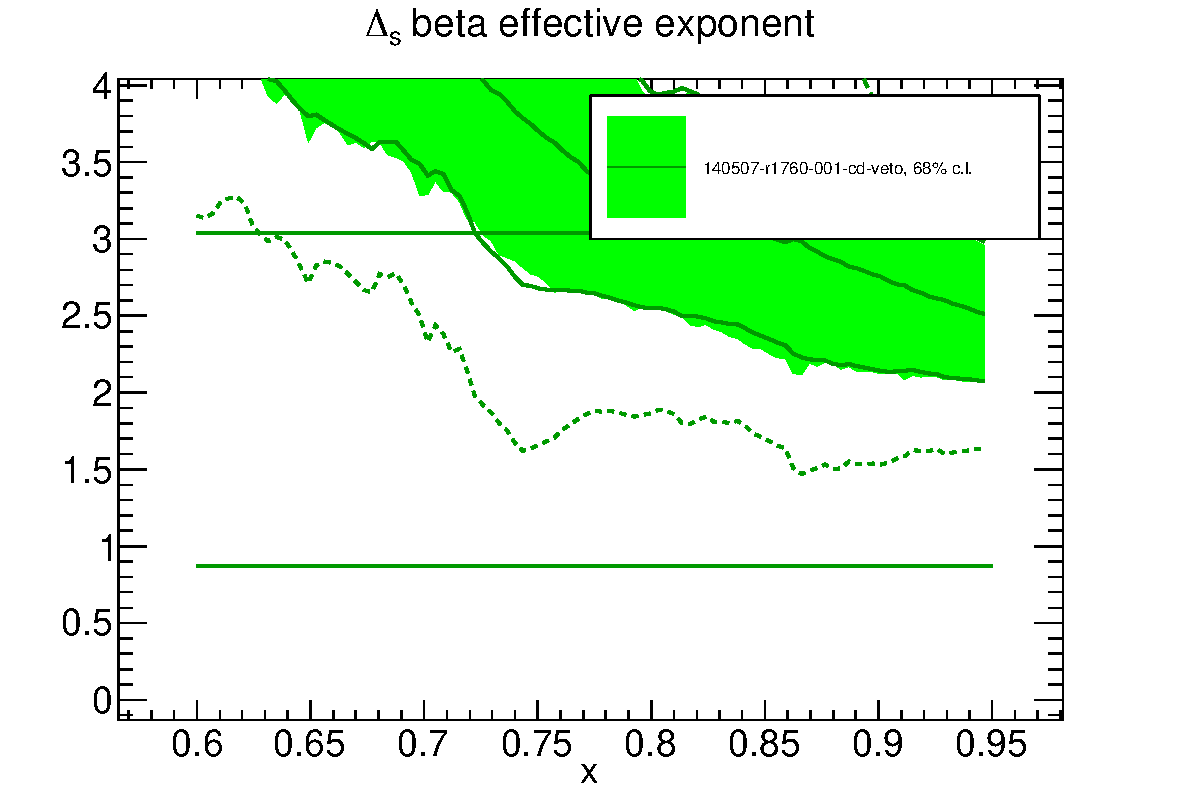
\includegraphics[width=0.42\textwidth]{7-PostLHC/figs/PreprocFixed/betapreproc_4.pdf}
%\caption[Impact of improved preprocessing range selection in the sea asymmetry PDF]{Impact of improved preprocessing range selection in the sea asymmetry PDF. The top figures demonstrate the $\Delta_s$ PDF obtained via a closure test to MSTW08 using the improved preprocessing procedure in green, with the underlying law shown in red. The figures below show the effective exponents for this PDF, and the effect of the improved range selection.}
%\label{fig:preproc3}
%\end{figure}
%\clearpage
%
%
%\begin{figure}[!]
%\centering
%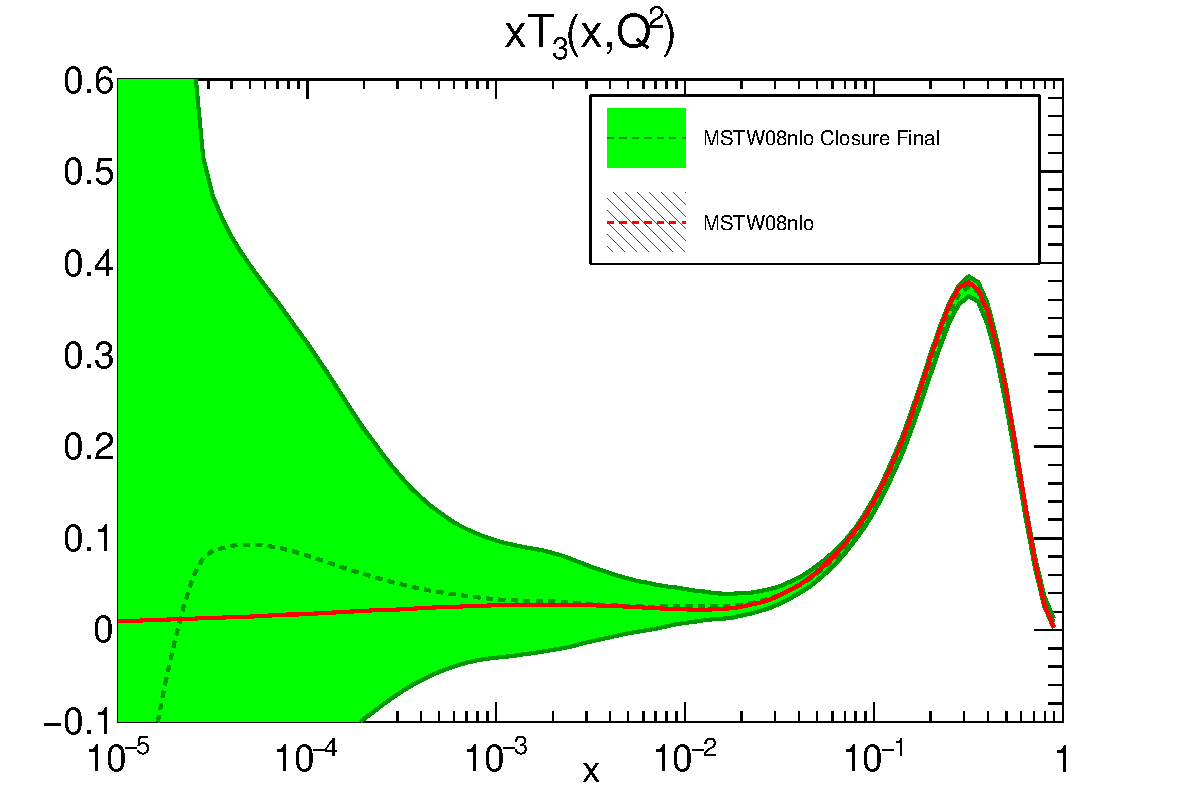
\includegraphics[width=0.42\textwidth]{7-PostLHC/figs/PreprocFixed/pdf_xT3_log_others.pdf}
%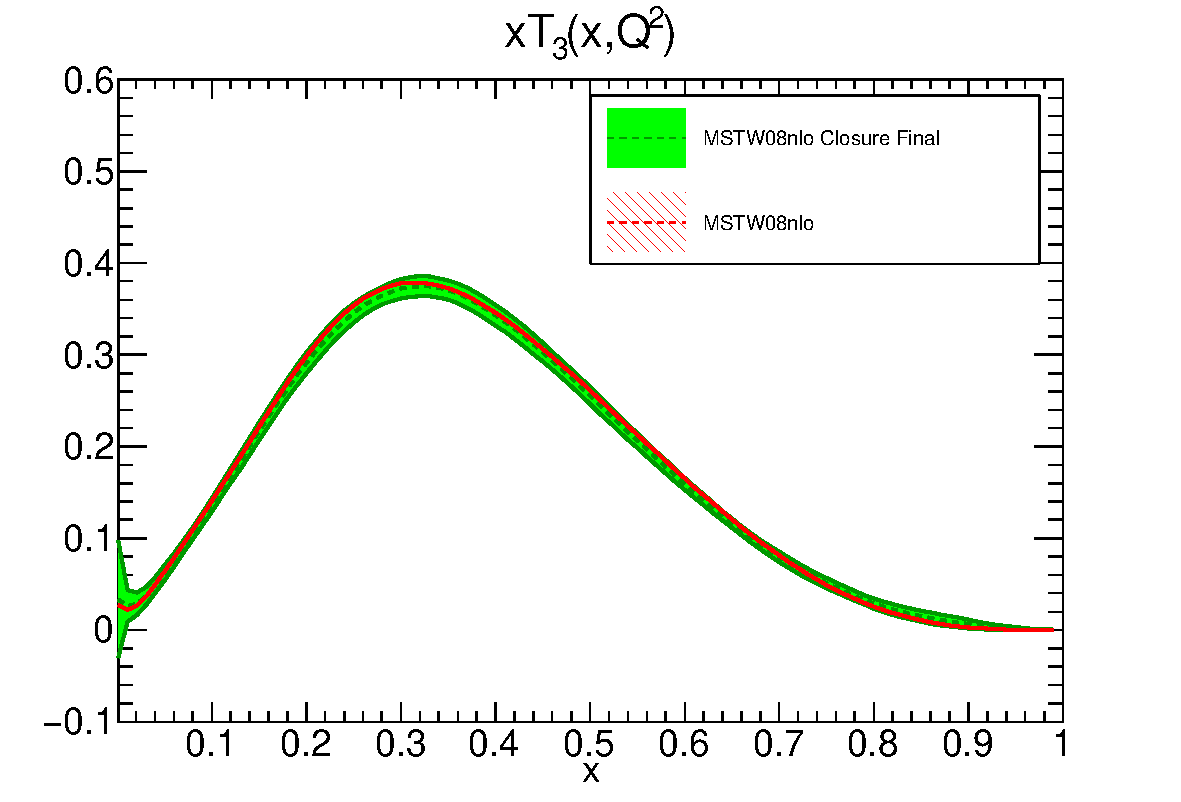
\includegraphics[width=0.42\textwidth]{7-PostLHC/figs/PreprocFixed/pdf_xT3_others.pdf}
%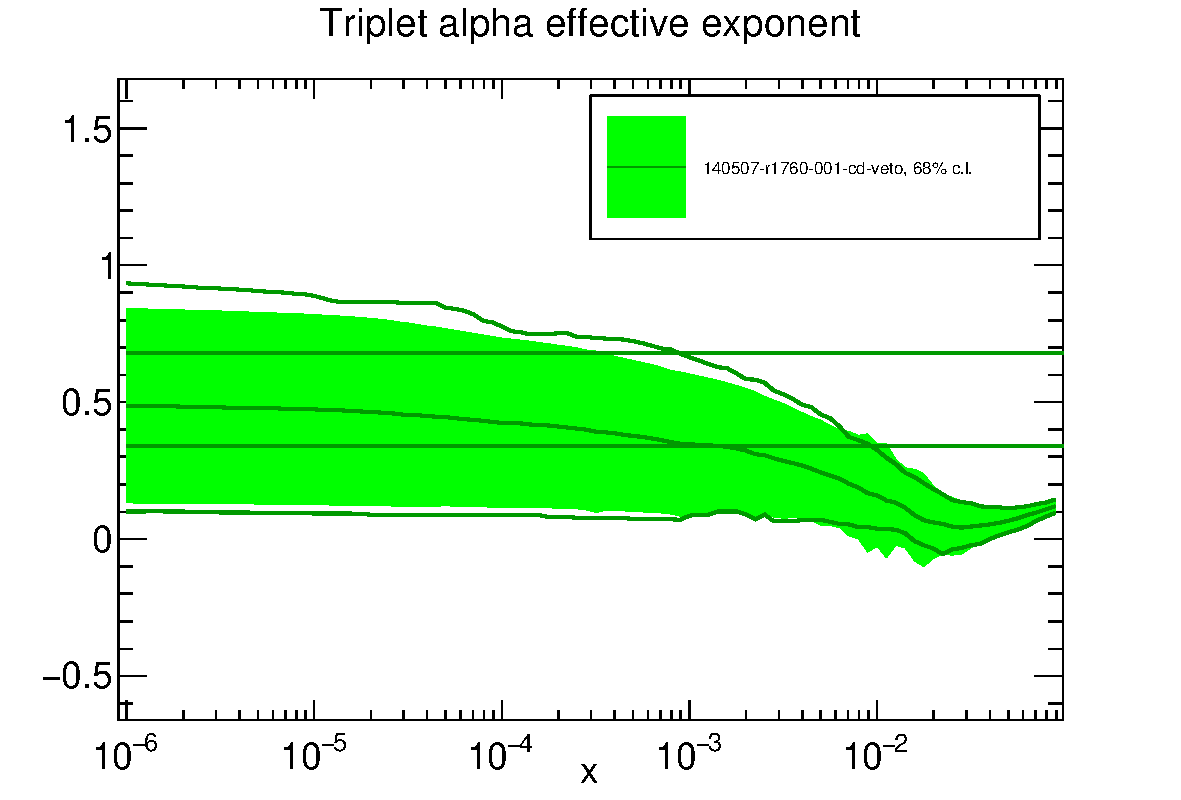
\includegraphics[width=0.42\textwidth]{7-PostLHC/figs/PreprocFixed/alphapreproc_3.pdf}
%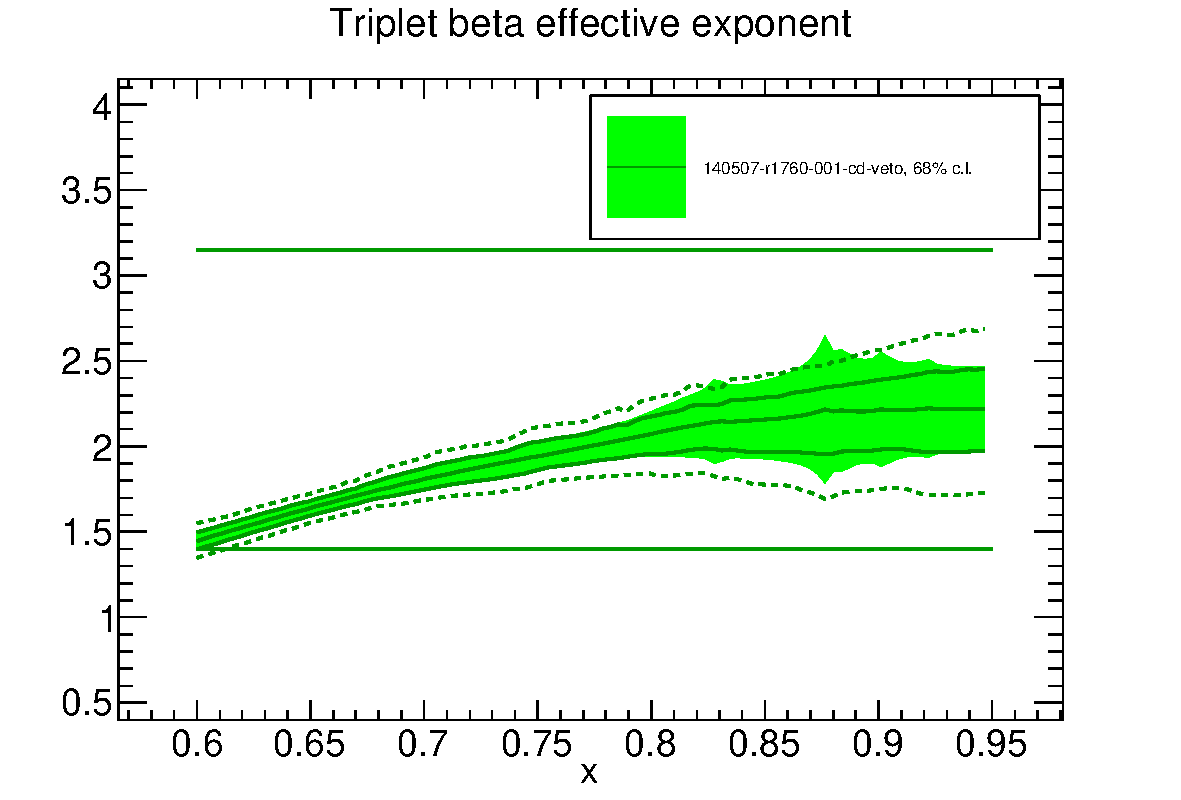
\includegraphics[width=0.42\textwidth]{7-PostLHC/figs/PreprocFixed/betapreproc_3.pdf}
%\caption[Impact of improved preprocessing range selection in the triplet PDF]{Impact of improved preprocessing range selection in the triplet PDF. Displayed as in Figure~\ref{fig:preproc3}. In the case of the high $x$ effective exponent, the data's preferred range lies well within the set randomisation range of the exponents. For the small-$x$ exponent, more iteration is needed here to settle on a larger range. The general features of the extended preprocessing ranges can be clearly seen in the top figures.}
%\label{fig:preproc4}
%\end{figure}

\subsection{Strange valence preprocessing}
A special case when considering the preprocessing of the neural networks is that of the strange valence distribution. As specified in Equation~\ref{eq:NNPDF23param}, the strange valence PDF in the NNPDF2.3 determination had an auxiliary term to encourage the PDF to perform its required sign change in the valence region. Such an additional term has been previously needed due to the lack of specific data constraints upon the strange valence distribution before the LHC, introducing a bias, albeit a physically motivated one. Additionally the auxiliary term provides a mechanism by which the strange valence sum rule may be imposed. In the NNPDF3.0 determination and beyond this auxiliary term has been removed given the enlarged dataset and it's improved sensitivity to the strange PDF.

Figure~\ref{fig:preproc5} demonstrates the effect of the removal of the strange auxiliary term upon a closure test fit to the MSTW08 set. While the NNPDF2.3 methodology closure fit struggles to accommodate the MSTW08 strange valence distribution, the updated methodology is able to reproduce the underlying law well, within enlarged uncertainties.

\begin{figure}[h!]
\centering
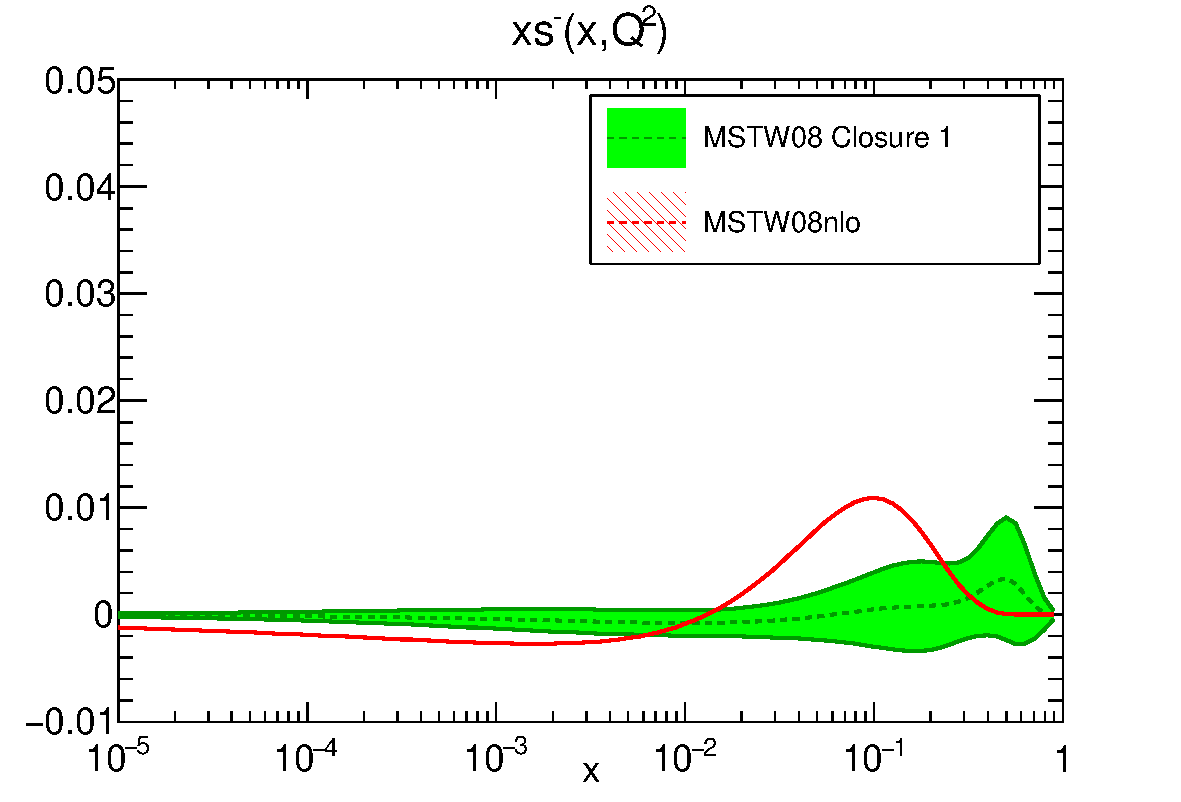
\includegraphics[width=0.42\textwidth]{7-PostLHC/figs/Preproc1/pdf_xsminus_log_others.pdf}
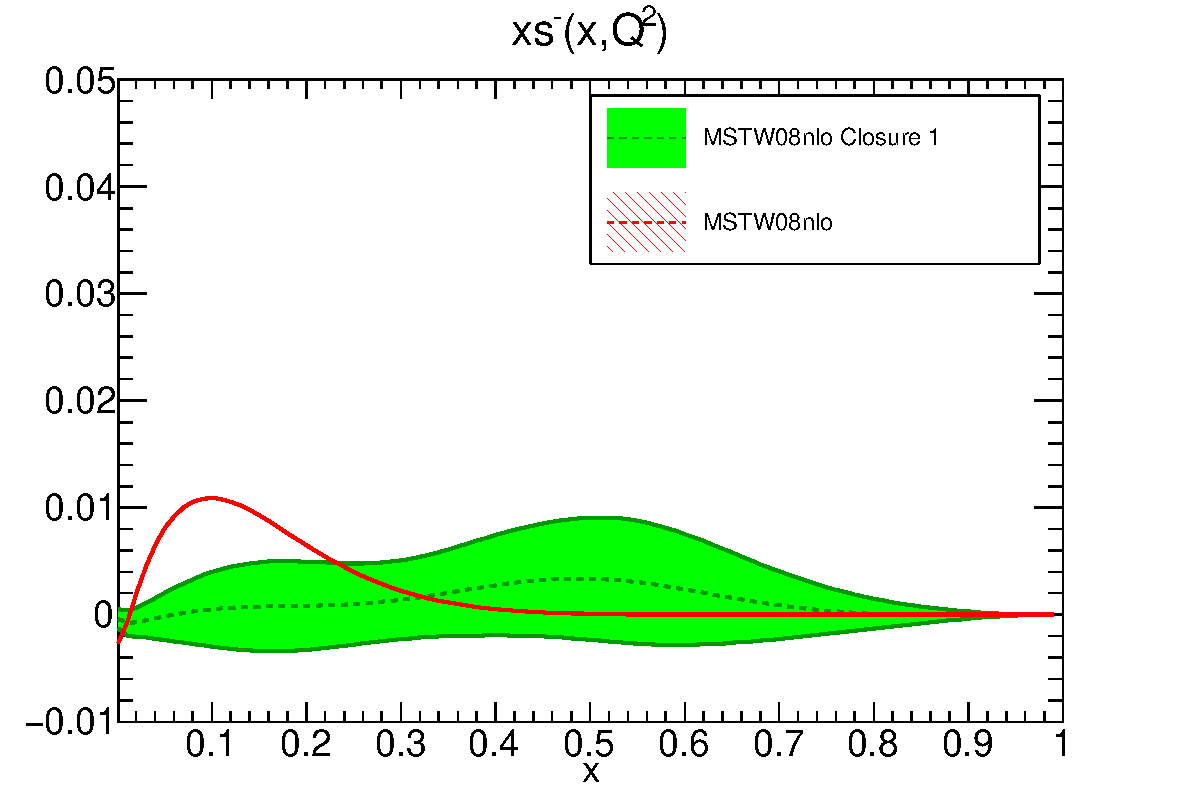
\includegraphics[width=0.42\textwidth]{7-PostLHC/figs/Preproc1/pdf_xsminus_others.pdf}
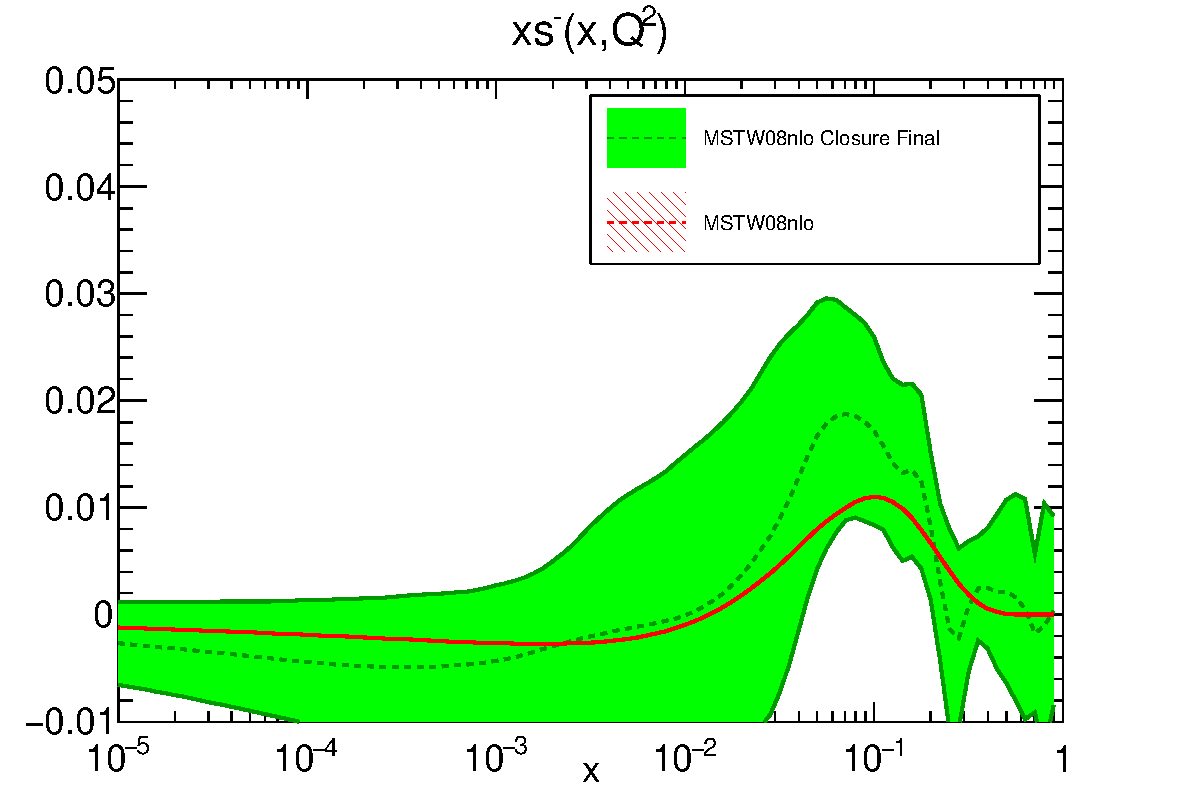
\includegraphics[width=0.42\textwidth]{7-PostLHC/figs/PreprocFixed/pdf_xsminus_log_others.pdf}
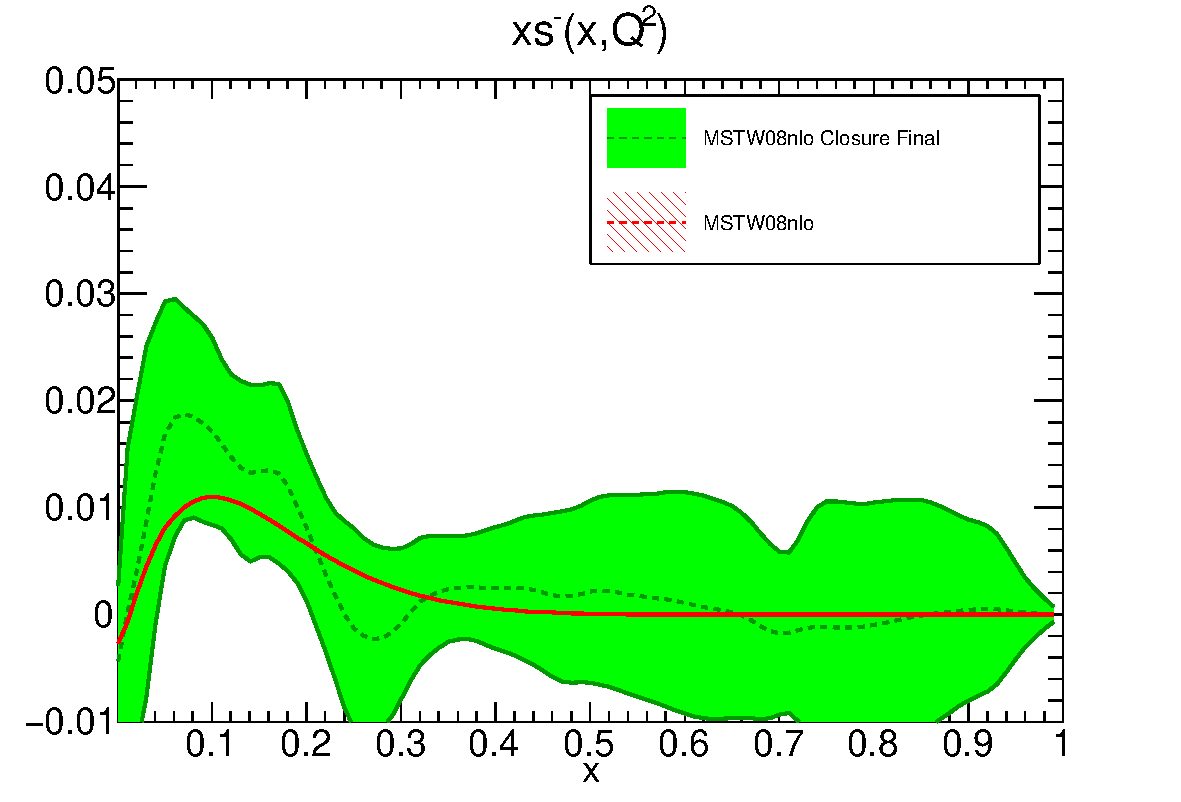
\includegraphics[width=0.42\textwidth]{7-PostLHC/figs/PreprocFixed/pdf_xsminus_others.pdf}
\caption[Impact of more flexible treatment of strange valence PDF in fits post NNPDF2.3]{Impact of more flexible treatment of strange valence PDF in fits post NNPDF2.3. The top two figures show a comparison of a closure test performed with the NNPDF2.3 preprocessing, and the figures below show the results using the more flexible parametrisation.}
\label{fig:preproc5}
\end{figure}

\clearpage

\section{PDF parametrisation}
The choice of PDF parameterisation and basis used in the fitting procedure has been reassessed with the help of the closure test procedure. In particular, a modification to the choice of fitting basis has been made necessary by the removal of the strange valence sum rule enforcing auxiliary term in the strange valence parametrisation. The most direct choice of fitting basis is the same basis as is used in PDF evolution, and therefore the basis required for PDFs in the {\tt FK} product. In this basis, the required quantum number sum rules may be applied as normalisations to the total valence, $V_3$ and $V_8$ distributions,
\ba V(x,Q^2_0) &=& N_V \left( u^- + d^-+ s^- \right)(x,Q^2_0),\nonumber \\
V_3(x,Q^2_0) &=& N_{V3} \left( u^- - d^- \right)(x,Q^2_0), \nonumber \\
V_8(x,Q^2_0) &=& N_{V8} \left( u^- + d^- - 2s^-\right)(x,Q^2_0),
\ea
where the normalisations $N$ are set such that
\ba \int_0^1 dx\, V(x,Q^2_0) &=& 3,\\
 \int_0^1 dx\, V_3(x,Q^2_0) &=& 1,\\
 \int_0^1 dx\, V_8(x,Q^2_0) &=& 3.\ea

In such a way, the total valence quantum number is fixed, along with the up, down and strange valence quantum numbers. The evolution basis also has the advantage of being
particularly efficient, not requiring any transformation before combination with {\tt FK} tables to calculate physical observables. We have shown, based upon closure test results, that the fit results
show a good degree of stability under such a change in parametrisation basis. While the previous strategy was designed to construct PDF combinations with specific data constraints, the flexibility of the fit
means that the results do not suffer when moving away from such a basis. Figure~\ref{fig:EVOLvs23BASIS} shows the statistical distance between a fit with the full evolution basis with a fit based upon the standard NNPDF2.3 parametrisation basis.
As expected, any differences are isolated to those PDFs whose parametrisation (and therefore preprocessing) has substantially changed e.g $\Delta_S$ and the strange PDFs. Even in these PDFs the differences are typically
less than half a standard deviation.


\begin{figure}[!]
\centering
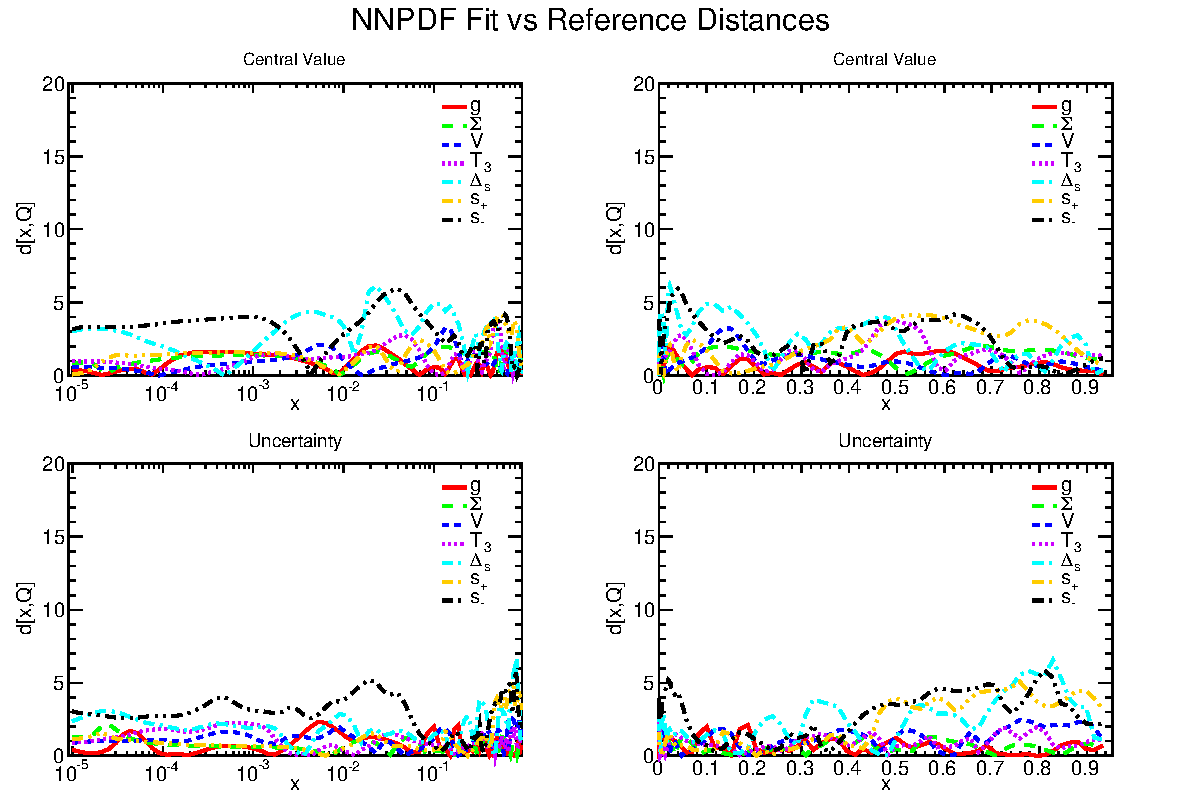
\includegraphics[width=0.9\textwidth]{7-PostLHC/figs/EVOLvs23BASIS/distances_evol.pdf}
\caption[Distance comparison of two closure test fits with differing parametrisation bases]{Distance comparison of two closure test fits with differing parametrisation bases. Distances are defined through the measure in Appendix~\ref{app:distances}, whereby a distance of 10 corresponds to $1\sigma$.}
\label{fig:EVOLvs23BASIS}
\end{figure}
  
\section{Minimisation and stopping}
In addition to examining areas where the choice of parametrisation may lead to some degree of bias, the closure test procedure is particularly useful for assessing the efficacy of a fitting methodology. Furthermore, the substantial gains in computational efficiency made in the transition to the {\tt nnpdf++} code mean that far more aggressive genetic minimisation strategies may be implemented.

The entirety of the NNPDF minimisation procedure has therefore been re-examined to ensure that it is the most effective methodology in the light of additional constraints coming from the LHC. Here we shall summarise some of the major modifications made since the NNPDF2.3 determination.

\subsection{Target weighted training}
Target Weighted Training (TWT) was a central feature of previous NNPDF determinations. TWT was developed in early NNPDF fits as a method of obtaining a balanced training across datasets, solving a problem with early neural network fits whereby some smaller datasets
were largely ignored by the minimisation in favour of larger, more constraining sets. This typically led to a very uneven fit quality profile over the complete experimental dataset. The TWT procedure solved this problem by introducing a training epoch at the beginning of a fit where each dataset had a target $\chi^2$. In the event where a fit iteration reached a $\chi^2$ value higher than the target, a large weight in fit quality was applied to that dataset in order to bring its fit quality down. 

While ensuring a relatively even training profile, the TWT procedure had a number of difficulties. The most important being the restriction of the early fit to a $\chi^2$ fit quality measure applied on a dataset-by-dataset basis, ignoring experimental uncertainty cross-correlations such as luminosity uncertainties, between datasets. Furthermore the TWT procedure introduced a considerable amount of complexity in the fitting procedure. With this in mind, real data fits with target weighted training were compared to fits without in the {\tt nnpdf++} framework with the large experimental dataset of NNPDF2.3 and updated genetic algorithm parameters. Figure~\ref{fig:twtvsnotwt} compares the dataset-by-dataset fit quality of two such example fits. With these fits we can see clearly that with a larger dataset and more efficient GA procedure, no large training imbalance can be seen in the fits even without the TWT procedure applied. Future NNPDF fits will therefore be performed without target weights, allowing for the consistent application of the experimental correlations across datasets throughout the fitting procedure.

\begin{figure}[!]
\centering
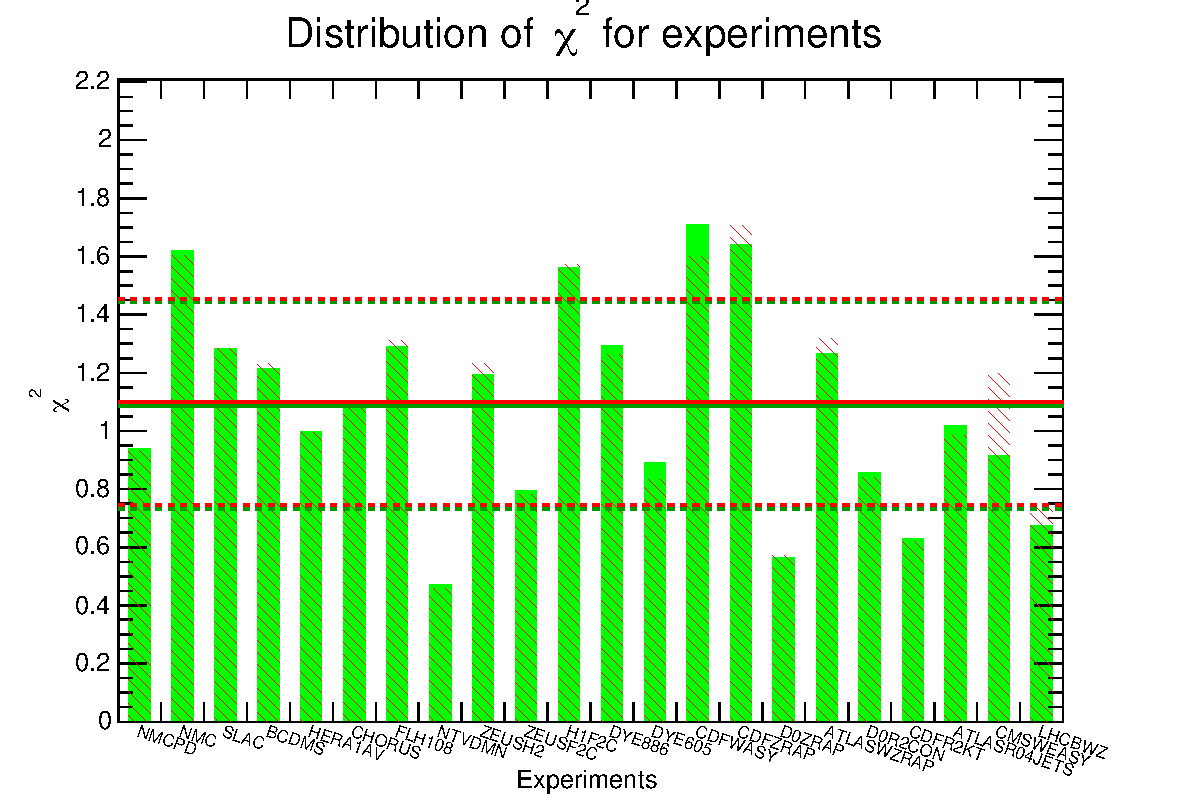
\includegraphics[width=1\textwidth]{7-PostLHC/figs/TWTvsnoTWT/chi2_histo.pdf}
\caption[Comparison of $\chi^2$ by dataset between real data fits with and without Target Weighted Training]{Comparison of $\chi^2$ by dataset between real data fits with (green bars) and without (red bars) Target Weighted Training.}
\label{fig:twtvsnotwt}
\end{figure}

\subsection{Genetic algorithm}
A number of changes have been made to the GA procedure used in NNPDF fits in order to improve fitting efficiency and provide more precise PDF determinations. In the analysis of the efficacy of a GA, level zero closure tests are particularly helpful in that they
directly test the ability of a minimisation procedure to reproduce a given function precisely. In these fits the closure test fit should be able to effectively draw a line between datapoints, leading to an ideal $\chi^2$ of zero to the pseudo-data.
%
%
%140430-r1753-001-sc.ini - DynStop
%140512-r1765-003-cd.ini  - LookBack 30k
%140512-r1765-004-cd.ini  - LookBack 60k
%
%
A number of modifications to the procedure have been tested, the most effective of which is the implementation of \emph{Nodal} mutations in the GA~\cite{Montana:1989:TFN:1623755.1623876}. In previous versions of the NNPDF GA, mutations were performed upon individual parameters of each neural network with no consideration as to their position in the network. 

The concept of nodal mutations introduces the strategy of mutating all parameters associated with a particular neural network \emph{node} at once. In this procedure a node of the network is chosen at random, then all of its associated weights connected to the earlier layer are mutated along with its threshold parameter. Doing so yields a much more effective genetic algorithm as demonstrated in the comparison in Figure~\ref{fig:nodalvsnonnodal}, where a standard GA is compared to a nodal mutation GA in their reproduction of the MSTW underlying law. The nodal GA is able to better resolve the underlying law, and to a greater precision. The comparison in Figure~\ref{fig:nodalvsnonnodal} is corroborated by the $\chi^2$ values of the two fits to the perfect pseudo-data in the level zero fit. The standard GA fit shown in the figure obtained a final $\chi^2$ of 0.0279 compared to 0.0043 for the nodal GA. The nodal GA strategy has therefore been adopted for future NNPDF determinations.

\begin{figure}[!]
\centering
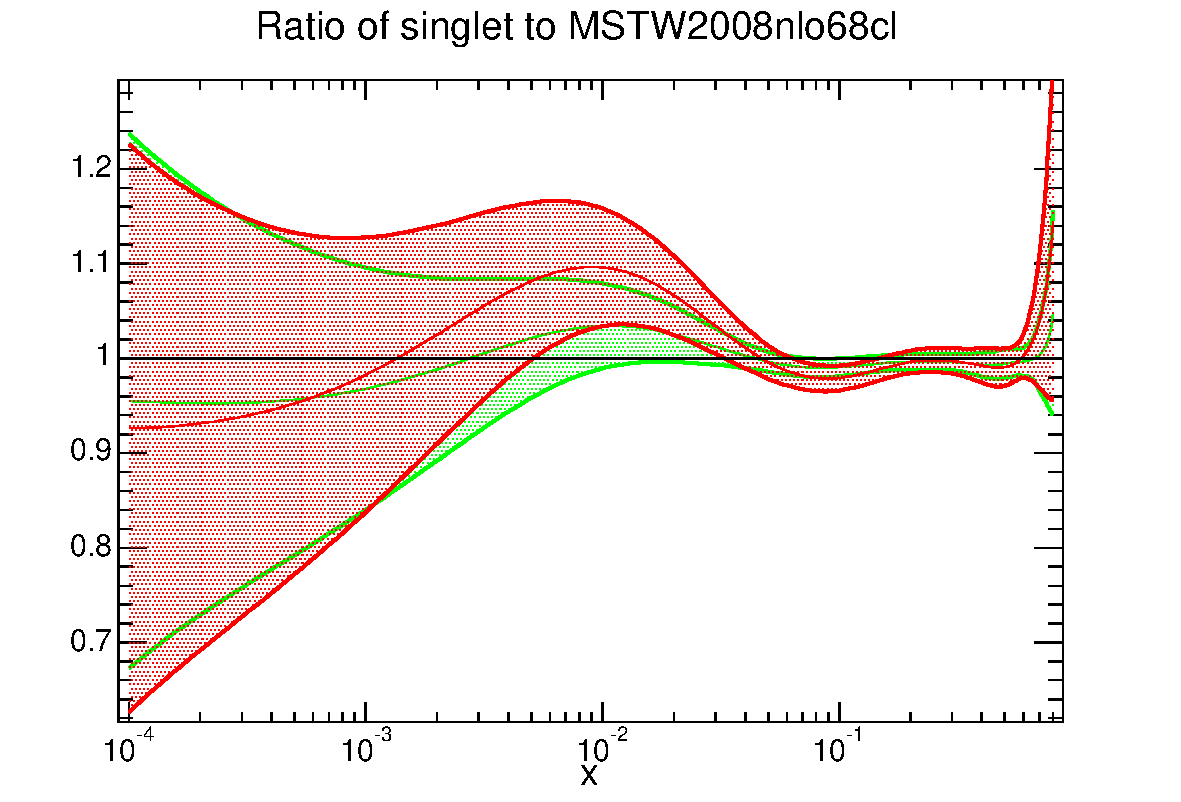
\includegraphics[width=0.48\textwidth]{7-PostLHC/figs/NodalGA/singlet.pdf}
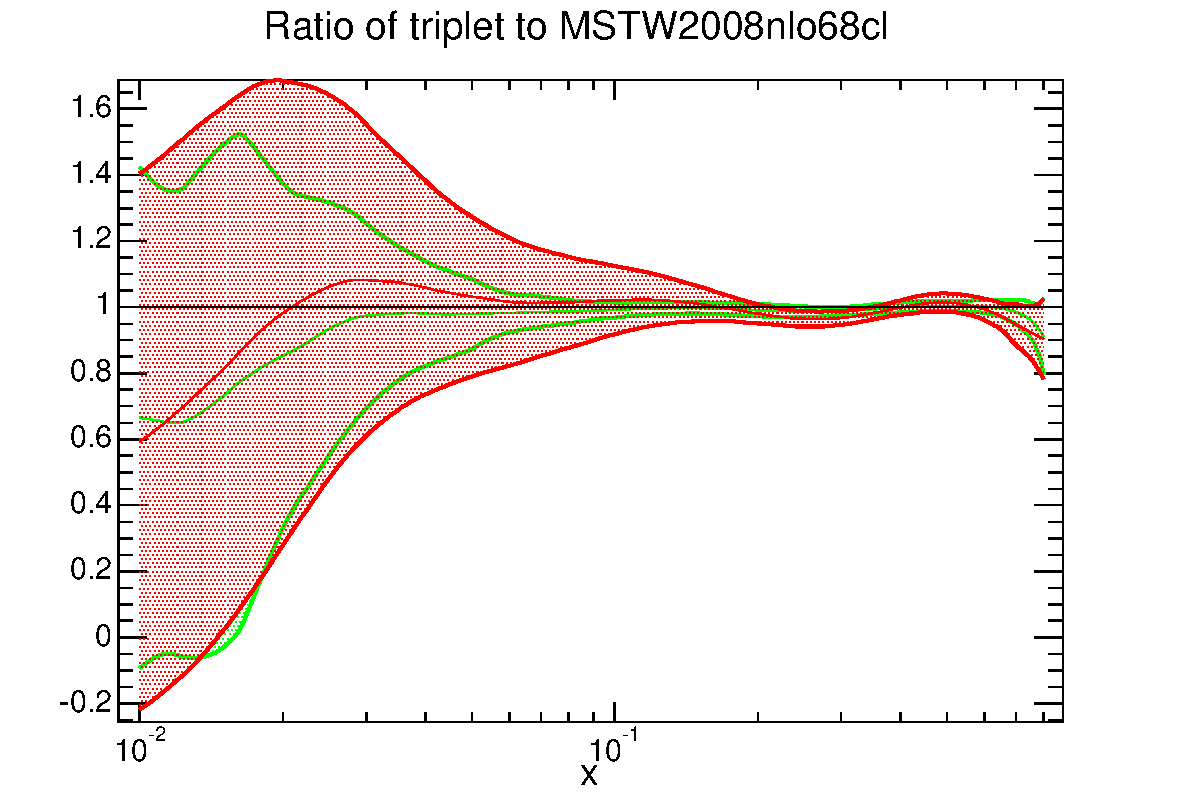
\includegraphics[width=0.48\textwidth]{7-PostLHC/figs/NodalGA/triplet.pdf}
\caption[Comparison of a conventional NNPDF GA fit with a Nodal GA fit in a closure test to MSTW2008]{Comparison of a conventional NNPDF GA fit (red bands) with a Nodal GA fit (green bands) in a closure test to MSTW08. PDFs are given as a ratio to the generating PDF set for the singlet (left) and triplet (right) distributions.}
\label{fig:nodalvsnonnodal}
\end{figure}

\subsection{Dynamical stopping}
The cross-validation dynamical stopping procedure utilised in previous {\tt FORTRAN} based NNPDF fits was triggered by a slope-detection algorithm applied to the fit quality profiles of each replica to the validation dataset. While providing a reasonable stopping criteria and preventing excessive overfitting, the relative balance between the degree of under- and over-learning was governed by the parameters of the slope-detection algorithm. Such sensitivity to the stopping parameters meant that a re-tune was often necessary upon large modifications to the dataset or minimisation algorithm. 

The modular nature of the stopping criteria implemented in the {\tt nnpdf++} framework means that alternative stopping procedures may be quickly and safely implemented to investigate their impact. One such stopping criterion that has demonstrated greater stability than the previous slope-detection based procedure is that of \emph{look-back} cross-validation. 

In this procedure all replicas are run for the maximum number of generations $N_{\text{gen}}^{\text{max}}$, all the while storing the GA generation that best described the validation dataset. At the end of the fit, the GA generation that minimised the $\chi^2$ to the validation set is selected as the best-fit stopping point, and that replica is used as a member of the Monte Carlo ensemble. This method yields an extremely clean stopping criterion, having no tuneable parameters aside from the maximum number of generations, and offers a very faithful implementation of the cross-validation method. Furthermore, the look-back procedure is not practically more time-consuming to implement despite running each replica to the maximum number of generations, as even in the previous dynamical stopping procedure the time taken to run a fit is typically given by the time taken by the slowest replica. In Figure~\ref{fig:LBCVchi2prof} the fit quality profile for a single PDF replica can be seen for the training and validation sets alongside the look-back stopping point. In this case, the look-back method can clearly discern an overlearning signal, as the fit quality to the validation set worsens while the training set $\chi^2$ improves.

\begin{figure}[!]
\centering
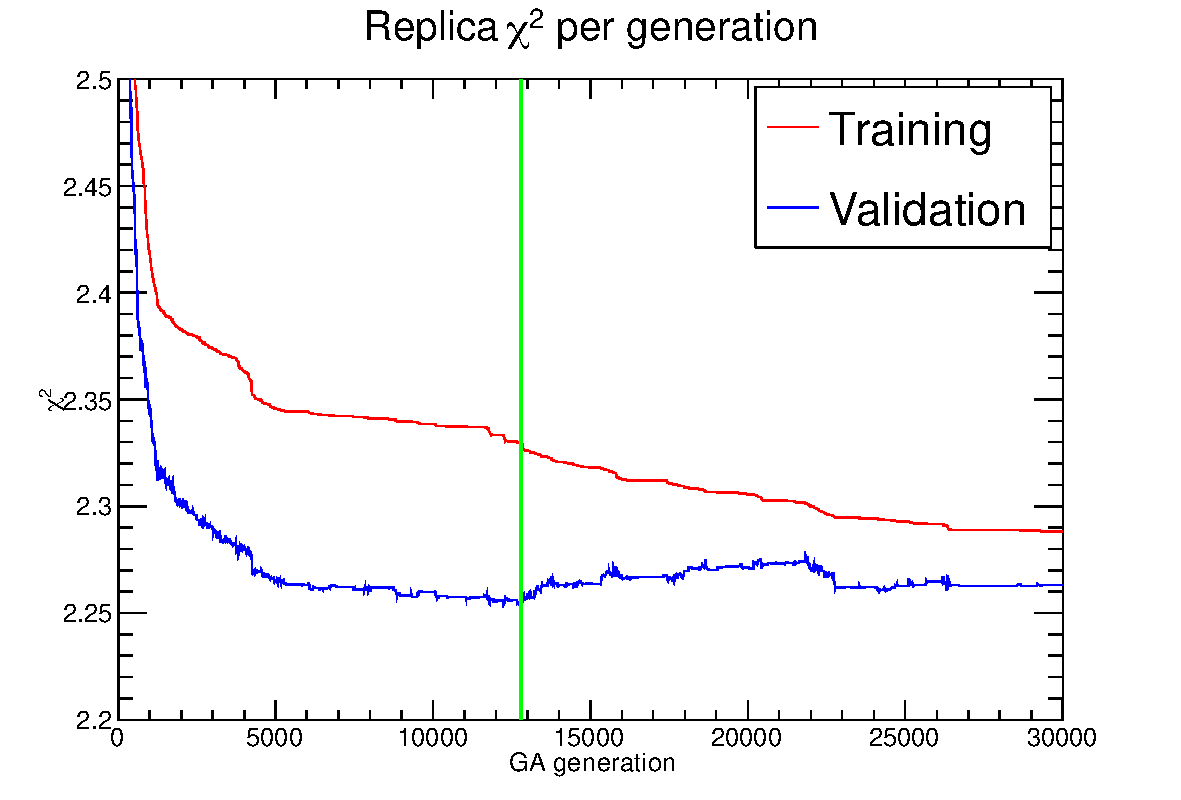
\includegraphics[width=0.7\textwidth]{7-PostLHC/figs/lookbackchi2prof.pdf}
\caption[Fit quality profiles for the training and validation sets in look-back cross validation]{Fit quality profiles for the training and validation sets in look-back cross validation. The red curve shows the fit quality to the training set, and the blue curve to the validation set as the number of fit generations goes on. The green line indicates the stopping point selected by the look-back criterion, generation 12813 having the minimum validation $\chi^2$.}
\label{fig:LBCVchi2prof}
\end{figure}


In Figure~\ref{fig:30kLBvsDYN} we compare the results for the singlet and gluon PDFs in the case of a look-back fit with $N_{\text{gen}}^\text{max}=$ 30,000 generations, and a fit with the NNPDF2.3 standard dynamical stopping. In both instances, the fit performed was a level two closure test using MSTW2008 as the underlying law. While differences are small the look-back fit demonstrates slightly smaller uncertainties, implying a marginal underlearning present in the NNPDF2.3 dynamical stopping procedure. The fits yield essentially equivalent results, although the optimal point determined in the look-back method is typically somewhat later than in the dynamical stopping as can be seen in the comparison of training length histograms in Figure~\ref{fig:30kLBvsDYNtl}. In this figure it is clear also that several PDF replicas in the look-back method stop close to the maximum number of generations available, implying that no significant overlearning can been resolved in their cases over the given GA interval.

In order to examine the effect of increasing the length of the look-back period, we compare the 30,000 generation fit to an extended 60,000 generation fit in Figure~\ref{fig:30kLBvs60kLB} where we use the PDF distance definition in Appendix~\ref{app:distances}. Distances of effectively zero throughout the PDF combinations and $x$-range mean that no change is observed between the two fits, demonstrating the stability of the method once a sufficiently large look-back length is used. The look-back cross-validation method as discussed here will therefore be implemented as the default stopping criterion for the NNPDF3.0 family of fits.


\begin{figure}[h!]
\centering
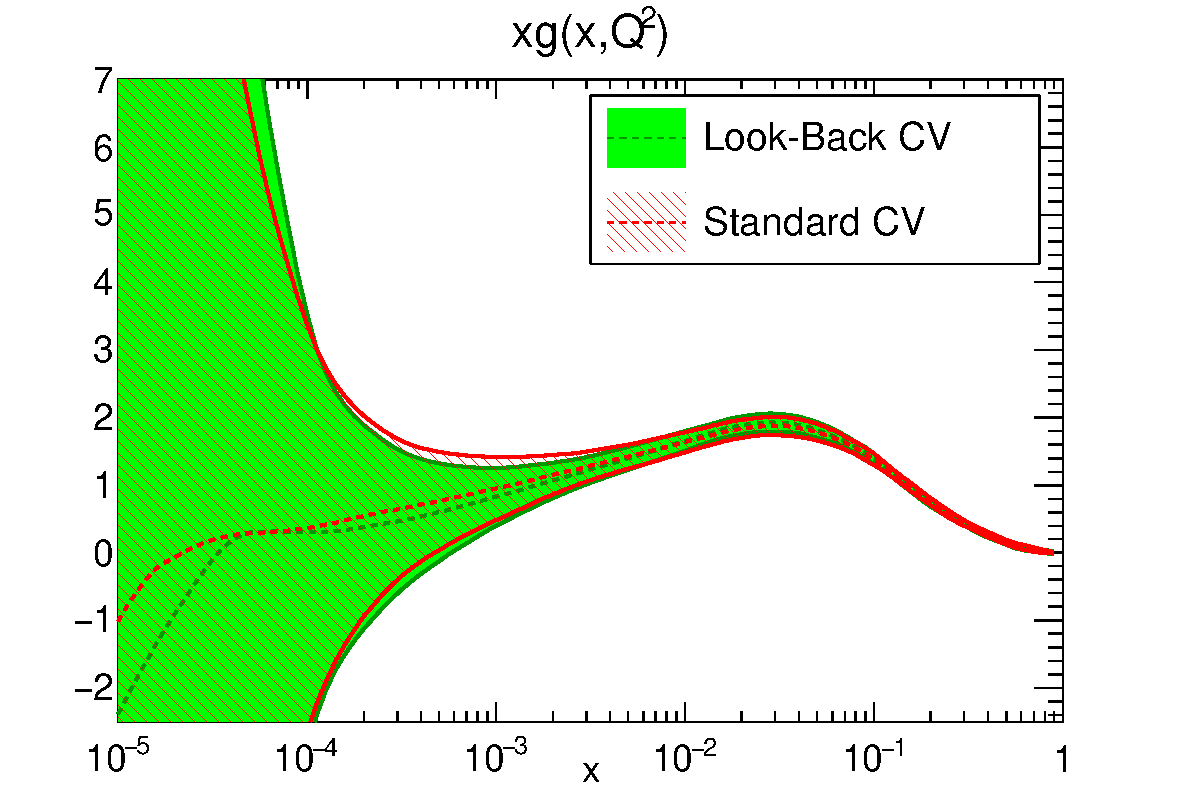
\includegraphics[width=0.48\textwidth]{7-PostLHC/figs/LB30kvsDYN/pdf_xg_log.pdf}
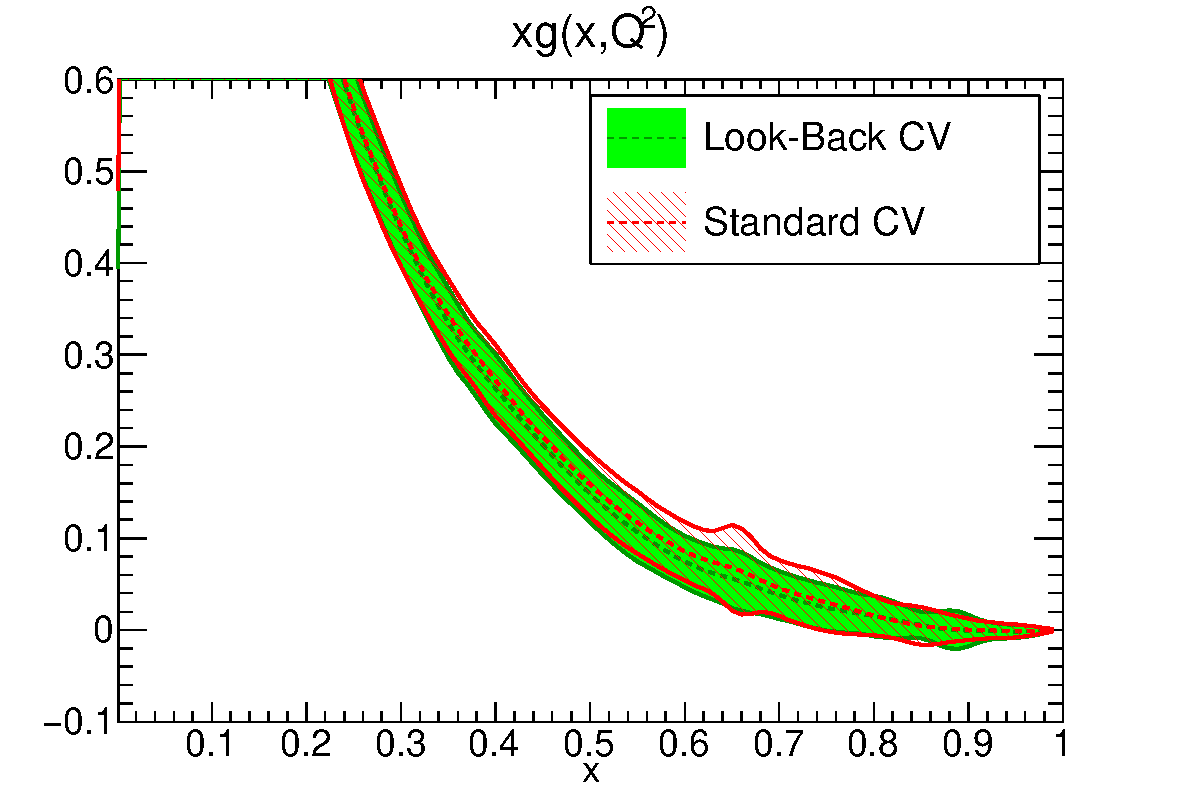
\includegraphics[width=0.48\textwidth]{7-PostLHC/figs/LB30kvsDYN/pdf_xg.pdf}\\
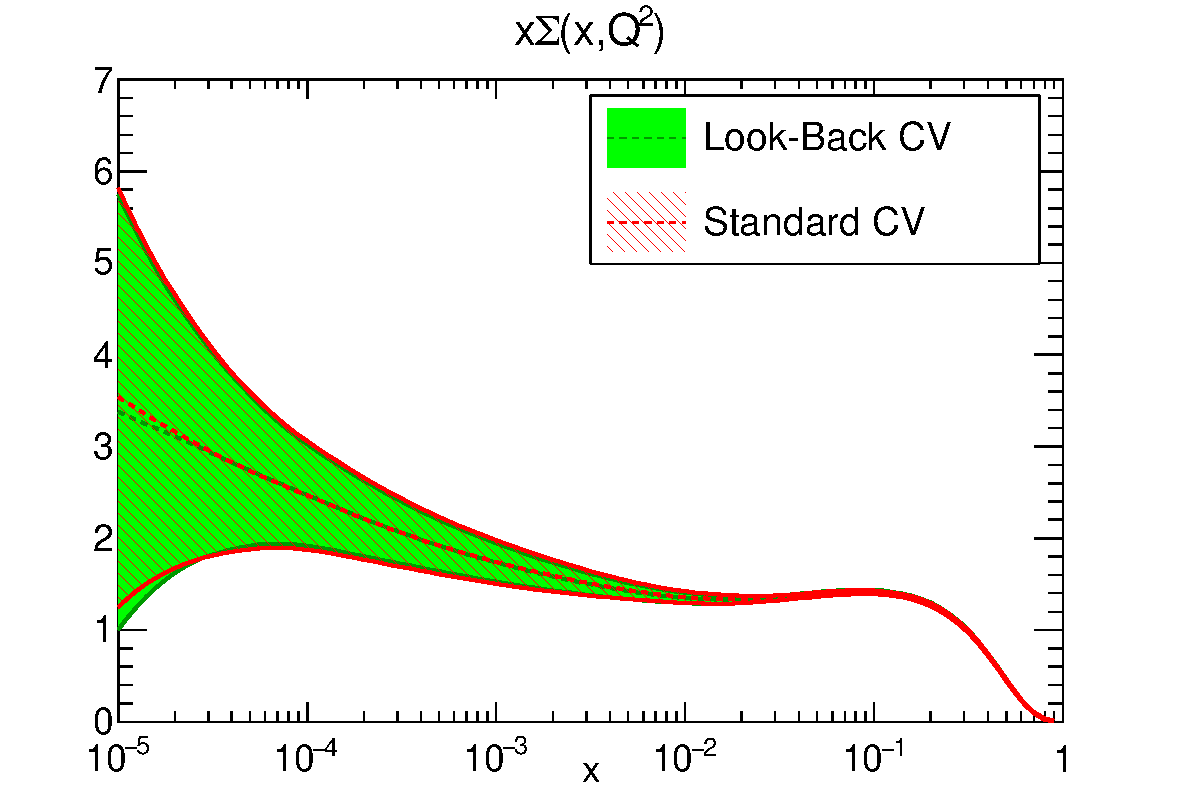
\includegraphics[width=0.48\textwidth]{7-PostLHC/figs/LB30kvsDYN/pdf_xsigma_log.pdf}
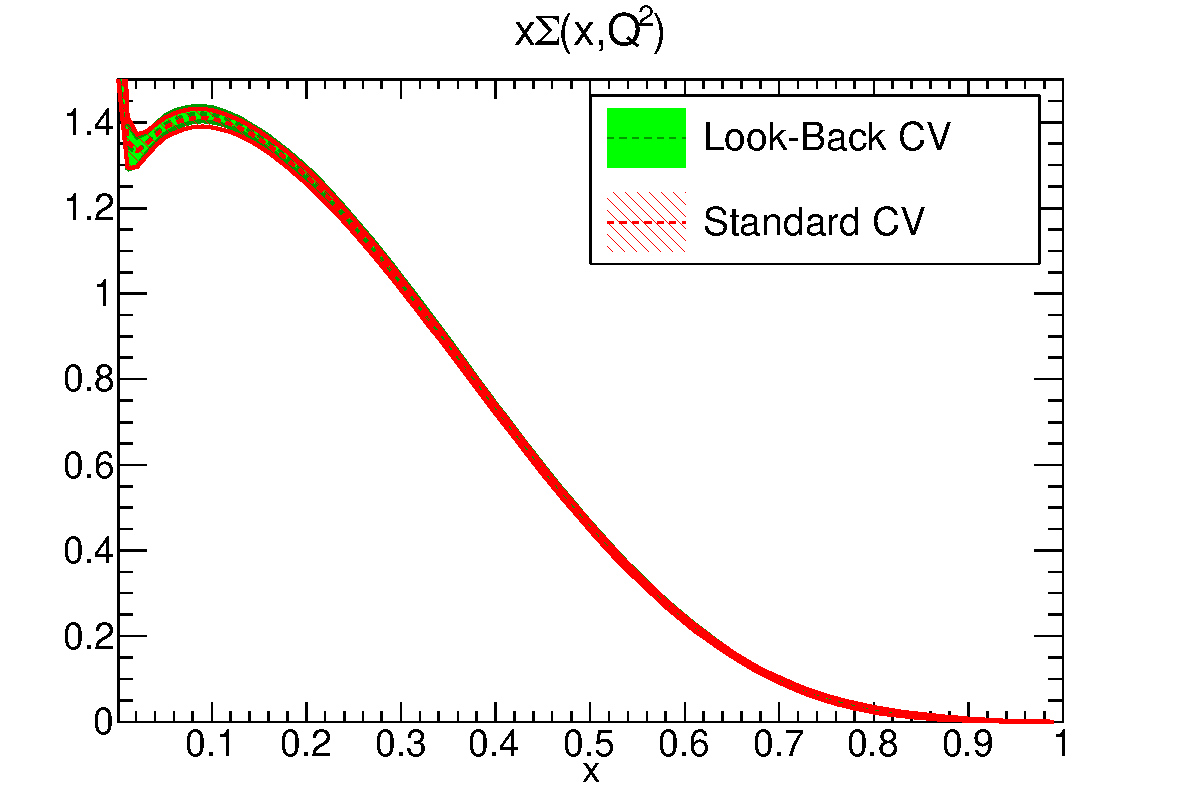
\includegraphics[width=0.48\textwidth]{7-PostLHC/figs/LB30kvsDYN/pdf_xsigma.pdf}
\caption[Comparison of PDFs obtained through look-back cross validation and NNPDF2.3 standard dynamical stopping]{Comparison of PDFs obtained through look-back cross validation and NNPDF2.3 standard dynamical stopping. PDFs for the singlet and gluon are shown, with green bands representing fits using the look-back method and red demonstrating those with the slope-detection algorithm used in NNPDF2.3 and earlier.}
\label{fig:30kLBvsDYN}
\end{figure}
 
  \begin{figure}[!]
\centering
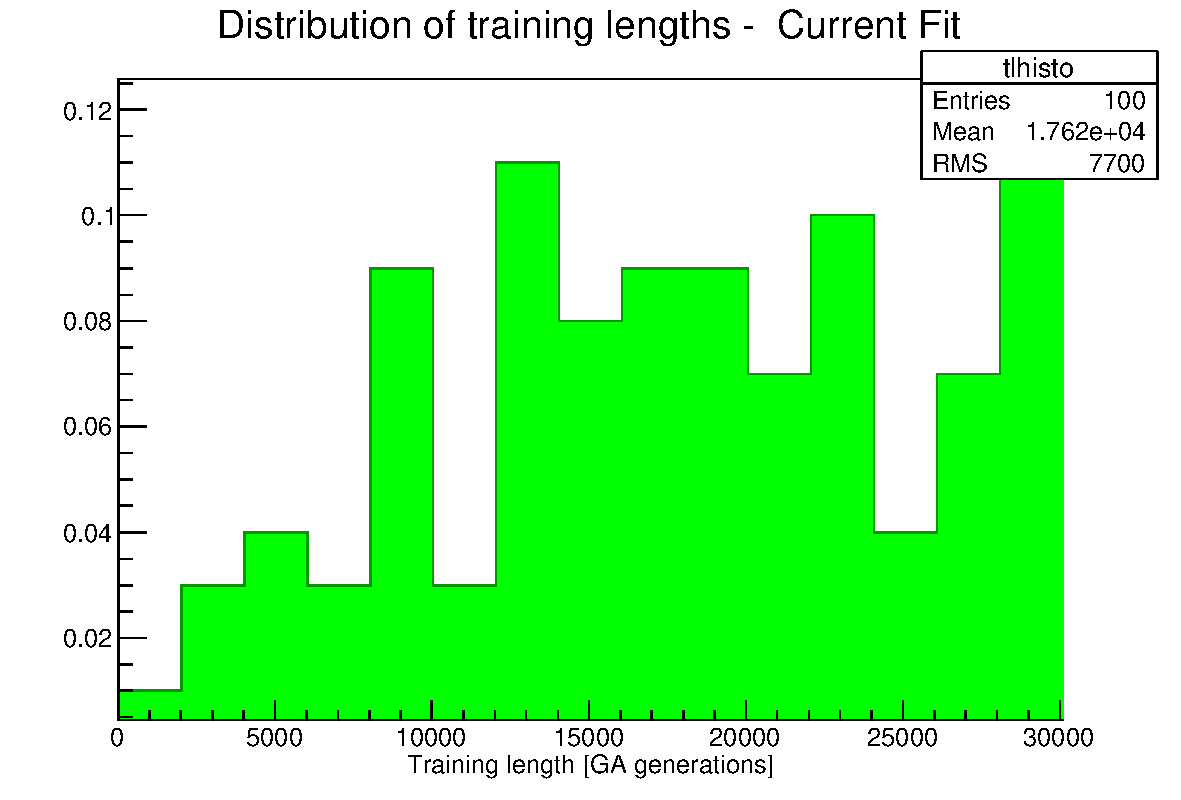
\includegraphics[width=0.48\textwidth]{7-PostLHC/figs/LB30kvsDYN/tl.pdf}
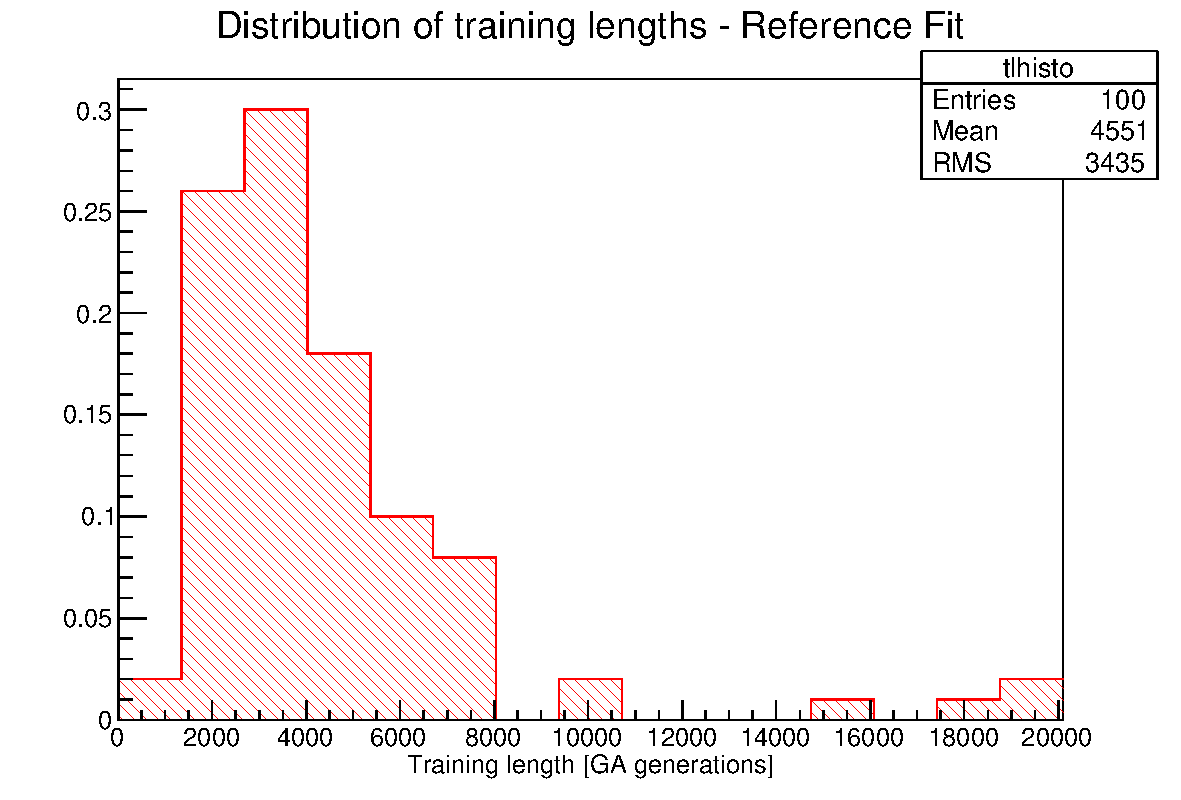
\includegraphics[width=0.48\textwidth]{7-PostLHC/figs/LB30kvsDYN/tl_ref.pdf}
\caption[Comparison of training lengths in look-back cross-validation and NNPDF2.3 standard dynamical stopping]{Comparison of training lengths in look-back cross-validation and NNPDF2.3 standard dynamical stopping. The left figure demonstrates the 'optimal point' determined by looking back over the while GA interval for the minimum validation $\chi^2$. The right figure shows the stopping point based upon the slope-detection algorithm.}
\label{fig:30kLBvsDYNtl}
\end{figure}

\begin{figure}[!]
\centering
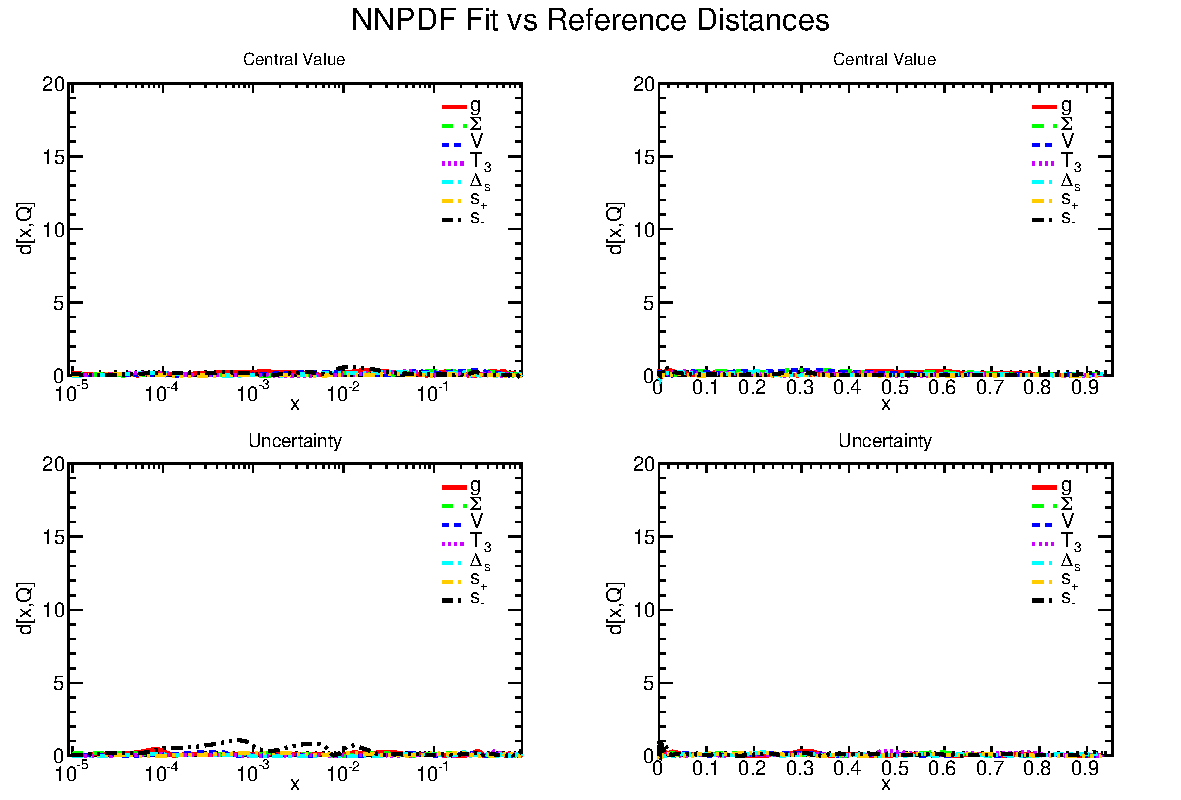
\includegraphics[width=0.9\textwidth]{7-PostLHC/figs/LB30kvsLB60k/distances_evol.pdf}
\caption[Distance comparison of two closure test fits with look-back stopping enabled and different maximum training lengths]{Distance comparison of two closure test fits with look-back stopping enabled and different maximum training lengths. Distances are computed between all evolution basis PDFs at the initial scale between $N_{\text{gen}}^\text{max}=$ 30,000 and $N_{\text{gen}}^\text{max}=$ 60,000 generation look-back fits.}
\label{fig:30kLBvs60kLB}
\end{figure}

\section{Methodology for NNPDF3.0}
We have performed an overview of the methodological developments made since the release of the NNPDF2.3 PDF set, with an aim to outline the procedure to be used in the forthcoming NNPDF3.0 set. To provide a stringent verification of the combined procedure, we shall now examine a set of closure test fits performed at various levels to differing generating PDF sets. In this section we present fits based upon a nodal genetic algorithm minimisation with look-back cross-validation stopping as detailed previously, with the iterative preprocessing procedure and new PDF fitting basis. Therefore the fits represent preliminary closure test results for the NNPDF3.0 methodology, upon a global pseudo-dataset of hadronic and DIS data. Results in this section will be presented using NLO calculations for the observables in the fit, although the conclusions will be very similar for an identical analysis at NNLO, as the closure test procedure is relatively insensitive to theory choices.

\subsection{Closure tests for NNPDF3.0}

Firstly let's consider the results obtained when fitting to an MSTW2008 generating PDF, the closure test guiding the methodological choices made so far in this section. In Figure~\ref{fig:finalClosure_MSTW} the ratio of the resulting closure test PDFs to the generating MSTW08 distributions are shown for some of the evolution basis PDFs. Here we show results for the kinematic region most constrained by the experimental pseudo-dataset: $10^{-2} \le x \le 1$. The level zero curves in Figure~\ref{fig:finalClosure_MSTW} closely reproduce the MSTW central values, achieving a final total $\chi^2/N_{\text{dat}} = 0.00182$. The uncertainty band in the case of the level zero result corresponds directly to the functional freedom available within the fitted pseudo-dataset. The level two fit clearly demonstrates the variations introduced by the simulated experimental noise, with the expected level of deviation clearly visible in the resulting PDFs. Given the simulated noise in the pseudo-dataset, the closure test still tracks the central value to an excellent level of accuracy, achieving an almost statistically ideal fit quality of $\chi^2/N_{\text{dat}} = 1.00021$.

As the preliminary NNPDF3.0 methodology has been validated against closure test fits to the MSTW2008 set, it is important to test the procedure's ability to reproduce a generating PDF with greater functional complexity. To verify the preliminary methodology in this case we now consider a closure test fit to the NNPDF2.3 PDF set. Figure~\ref{fig:finalClosure_NNPDF} demonstrates once more the level zero and two closure test fits to NNPDF2.3. Even given the greater functional freedom present in the previous NNPDF determination, the 3.0 closure test provides an excellent reproduction of the generating functions, with fit qualities of  $\chi^2/N_{\text{dat}} = 0.00287$ and $1.01356$ respectively. Once again the uncertainty due to parametrisation flexibility is demonstrated in the level zero fit, while the level two fit provides a closer simulation of a full fledged experimental data fit. These figures therefore suggest that the preliminary NNPDF3.0 methodological choices can accurately determine complex functional forms without any modification with respect to fits to much simpler parametrisations.

For a final closure test, we shall now consider a fit using the CT10 PDF set as a set of generating functions. In this way we can verify the NNPDF3.0 method in a way that is independent of the closure PDF set guiding the methodological development (MSTW2008) and previous NNPDF determinations. The results of the test, once more at level zero and two, are shown in Figure~\ref{fig:finalClosure_CT10}. The closure test fit provides once again an excellent description of data, with $\chi^2/N_{\text{dat}} = 0.00130$ for the level zero fit and $1.01324$ for the level one. The procedure detailed here has now been validated against three different generating PDFs in a closure test and is able to convincingly reproduce the generating sets in each of them. We can therefore be confident that when applied to real experimental data the procedure will yield an accurate result up to theoretical uncertainties.

\begin{figure}[!]
\centering
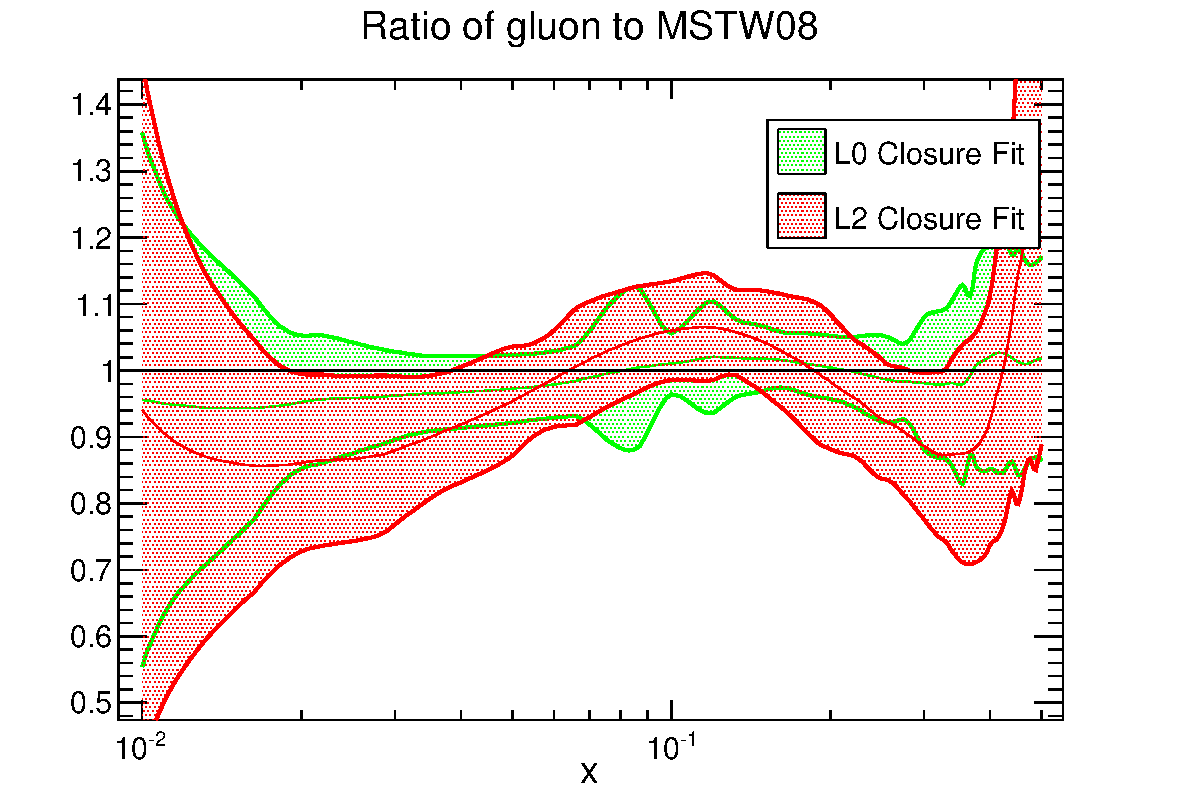
\includegraphics[width=0.45\textwidth]{7-PostLHC/figs/finalClosure/MSTW0/gluon.pdf}
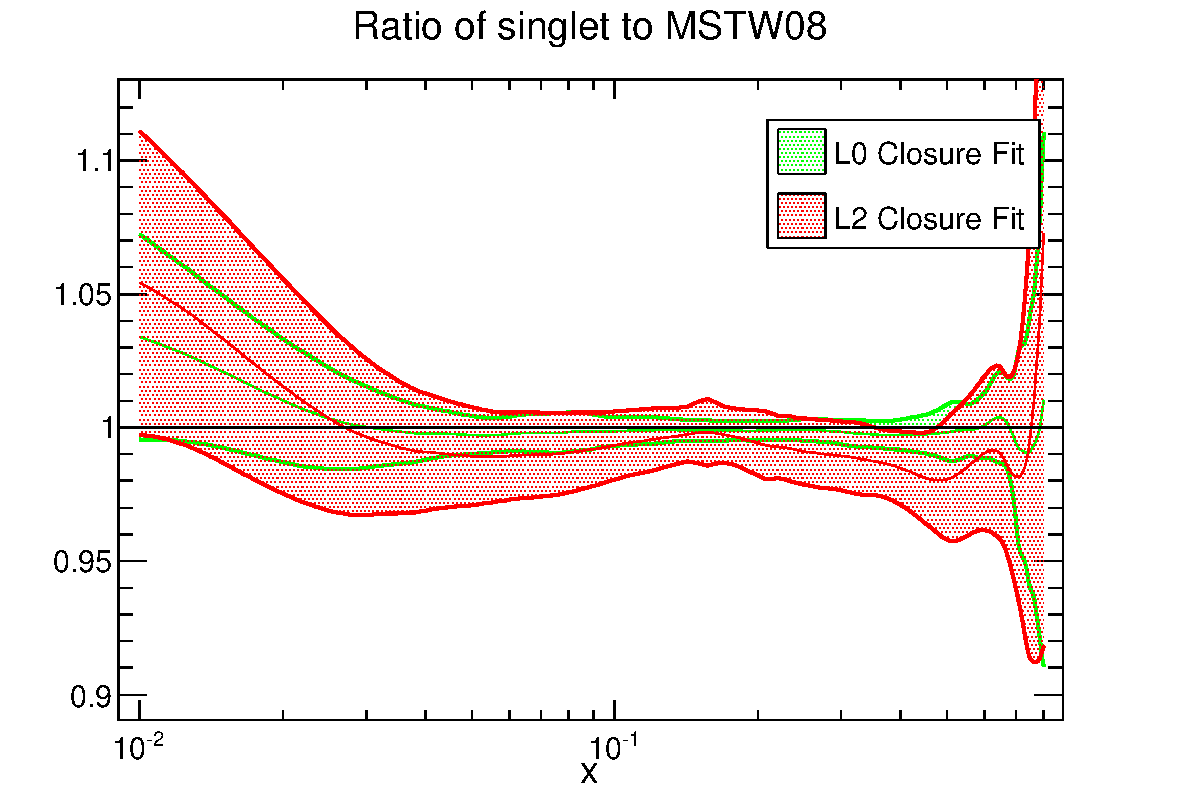
\includegraphics[width=0.45\textwidth]{7-PostLHC/figs/finalClosure/MSTW0/singlet.pdf}
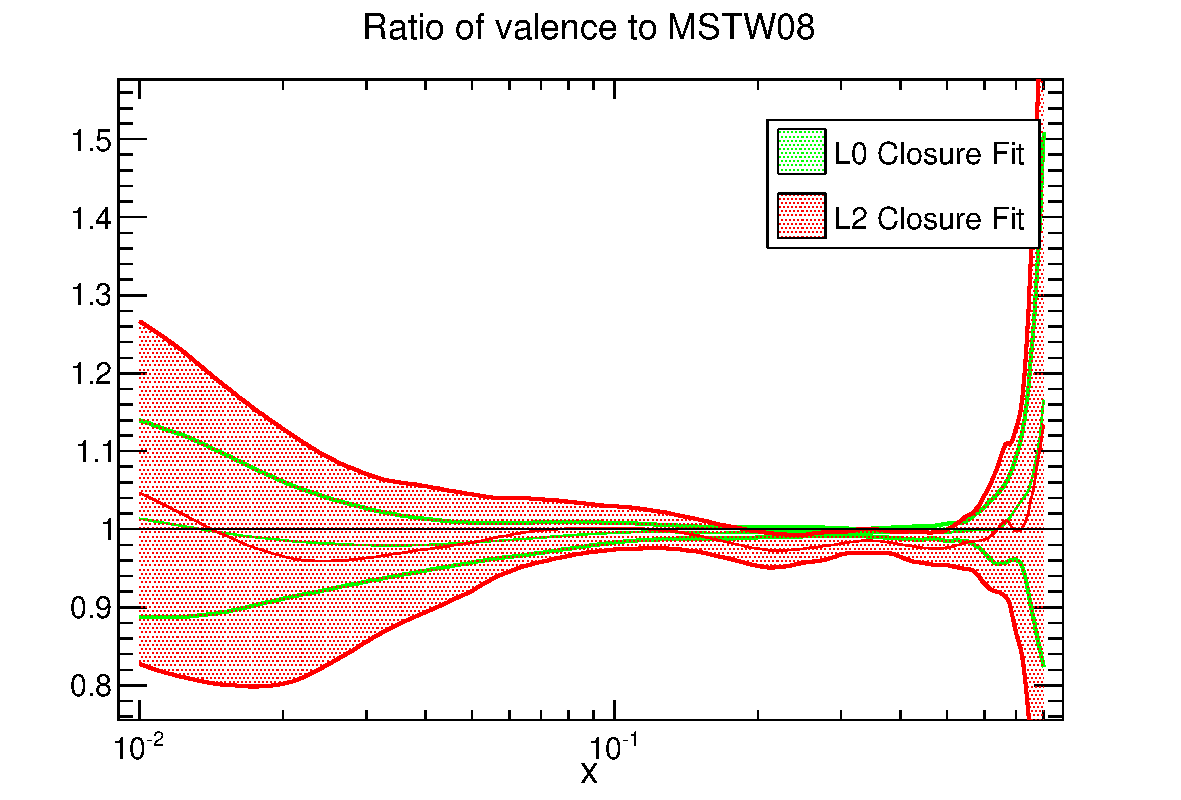
\includegraphics[width=0.45\textwidth]{7-PostLHC/figs/finalClosure/MSTW0/valence.pdf}
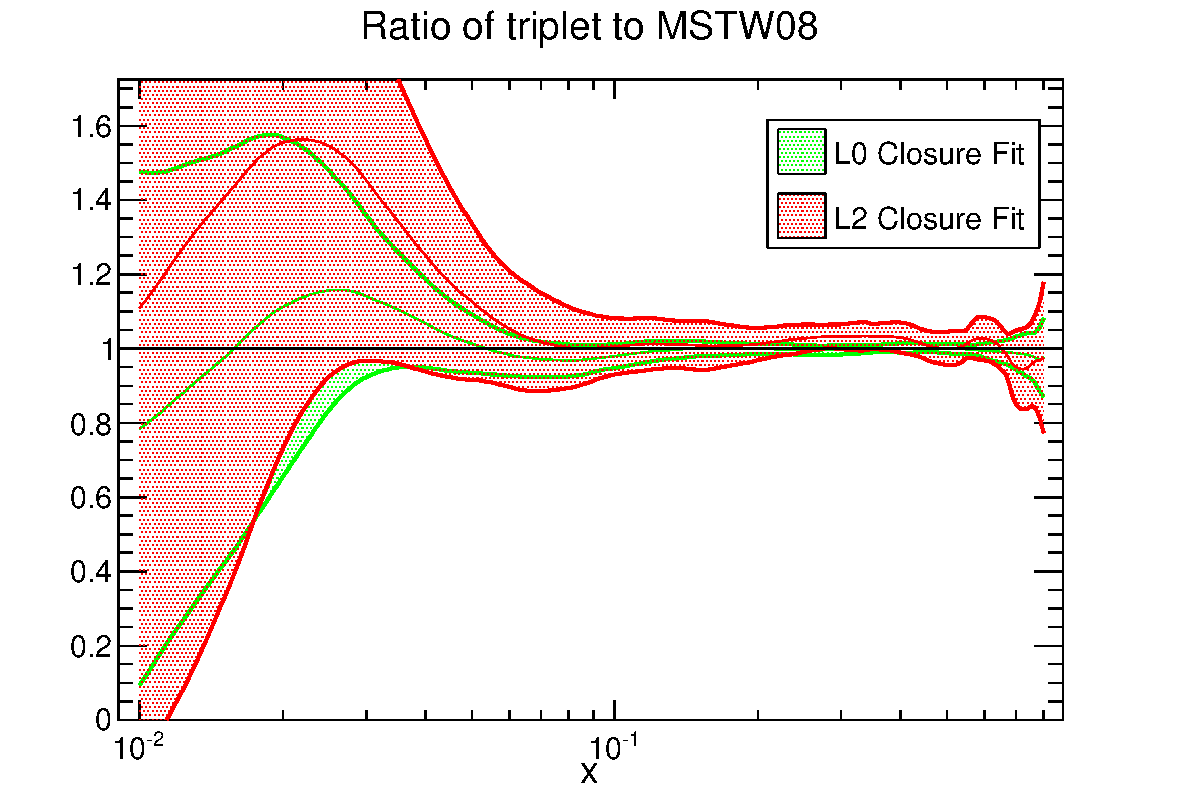
\includegraphics[width=0.45\textwidth]{7-PostLHC/figs/finalClosure/MSTW0/triplet.pdf}
\caption[NNPDF3.0 methodology closure test fit to MSTW2008 NLO]{NNPDF3.0 methodology closure test fit to MSTW2008 NLO. Curves are shown normalised to the generating PDF for the gluon, singlet, triplet and valence distributions. The green curves show the results of a level zero closure test, while the red curves show the results of a level two test.}
\label{fig:finalClosure_MSTW}
\end{figure}
\begin{figure}[!]
\centering
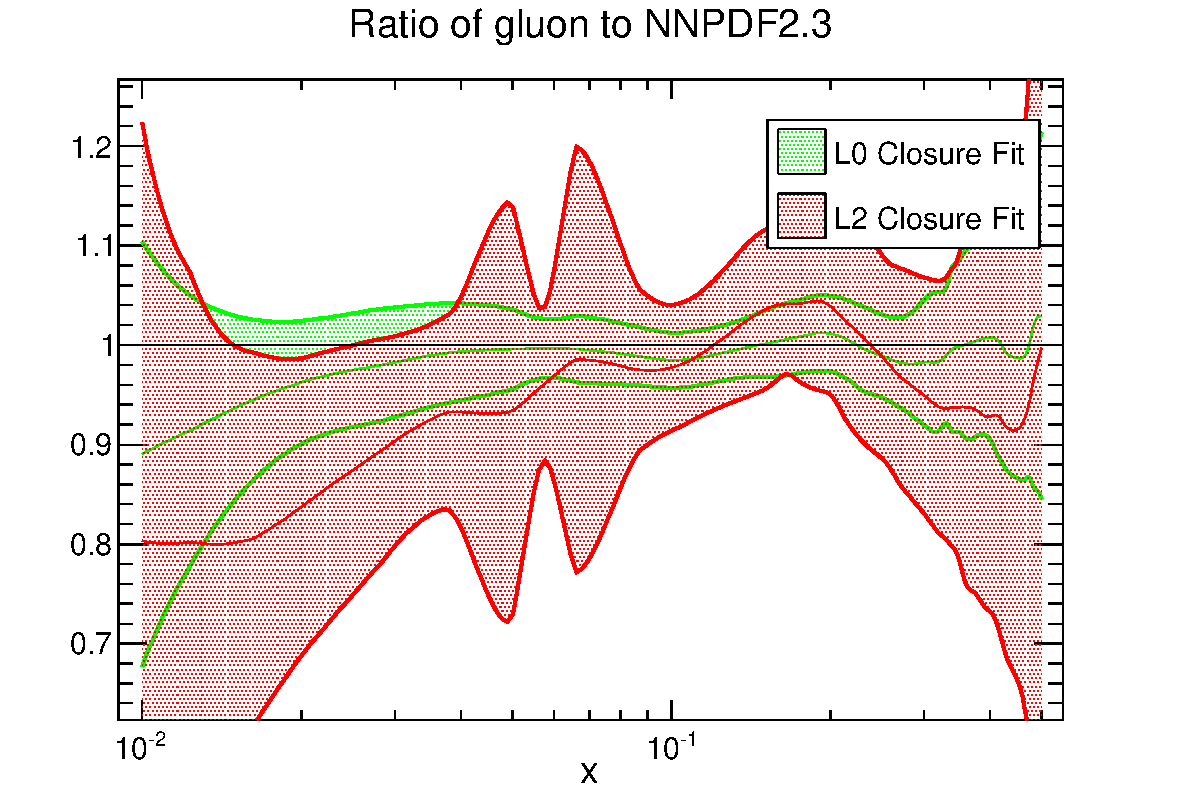
\includegraphics[width=0.45\textwidth]{7-PostLHC/figs/finalClosure/NNPDF23/gluon.pdf}
\includegraphics[width=0.45\textwidth]{7-PostLHC/figs/finalClosure/NNPDF23/singlet.pdf}
\includegraphics[width=0.45\textwidth]{7-PostLHC/figs/finalClosure/NNPDF23/valence.pdf}
\includegraphics[width=0.45\textwidth]{7-PostLHC/figs/finalClosure/NNPDF23/triplet.pdf}
\caption[NNPDF3.0 methodology closure test fit to NNPDF2.3 NLO]{NNPDF3.0 methodology closure test fit to NNPDF2.3 NLO. Plots as in Figure~\ref{fig:finalClosure_MSTW}. }
\label{fig:finalClosure_NNPDF}
\end{figure}
\begin{figure}[!]
\centering
\includegraphics[width=0.45\textwidth]{7-PostLHC/figs/finalClosure/CT10/gluon.pdf}
\includegraphics[width=0.45\textwidth]{7-PostLHC/figs/finalClosure/CT10/singlet.pdf}
\includegraphics[width=0.45\textwidth]{7-PostLHC/figs/finalClosure/CT10/valence.pdf}
\includegraphics[width=0.45\textwidth]{7-PostLHC/figs/finalClosure/CT10/triplet.pdf}
\caption[NNPDF3.0 methodology closure test fit to CT10 NLO]{NNPDF3.0 methodology closure test fit to CT10 NLO. Plots as in Figure~\ref{fig:finalClosure_MSTW}. }
\label{fig:finalClosure_CT10}
\end{figure}

\subsection{Improvements in data fits for NNPDF3.0}
While we have now validated much of the methodology to be used in the NNPDF3.0 determination, we shall now finally investigate some of the expected differences arising with respect to the NNPDF2.3 results in the case of a fit to experimental data. In order to directly assess the changes arising purely from the methodological differences in the two approaches, we shall perform two fits to a small common dataset, one with the full NNPDF2.3 machinery and the second with the improvements implemented in the NNPDF3.0 procedure. It should be noted that these results are of an extremely preliminary nature and as so should only be taken as roughly indicative of the final results. Furthermore, the full NNPDF3.0 set will benefit from a considerably expanded dataset with respect to the NNPDF2.3 determination. 

For these test fits, we use a collider-only dataset to ensure a maximally consistent set of experimental data, including the full NNPDF2.3 LHC and Tevatron datasets, and the HERA-1 combined DIS results. Once more, the fits were run with a maximum number of generations of $N_{\text{gen}} = 30,000$. The NNPDF2.3-like fit was otherwise performed according to the settings of the central NNPDF2.3 fit. The NNPDF3.0 fits were performed with identical settings to the closure test fits described in the previous section. 

Looking firstly at the gluon and singlet sectors, in Figure~\ref{fig:23vs30methodology_1} we see the results of the two methodology test fits compared as a ratio to the NNPDF2.3 methodology fit's central value. The first feature to note is that in the region where data constraints in this test fit are largest, the two methodologies remain very consistent in their results, with the most significant changes occurring in the extrapolation regions and for the large-$x$ singlet. At small-$x$ the NNPDF3.0 methodology fit is more confident in the extrapolation for both singlet and gluon PDFs, resulting in a systematically smaller uncertainty. At large-$x$ there is a moderate shift in the gluon central value in the NNPDF3.0 result, and a broadening of uncertainties. The same pattern can be found in the large-$x$ gluon, where once again uncertainties are slightly larger and there is some change in central value. However both distributions remain in agreement within their uncertainties, validating that the two methodologies remain compatible within the experimental uncertainty present in the test dataset.

To investigate the impact of the methodological changes to PDFs sensitive to the valence distributions and quark flavour separation, we plot the valence and triplet PDF combinations in Figure~\ref{fig:23vs30methodology_2}. In the valence PDF comparison, we see a similar pattern as for the singlet and gluon PDFs, where the low-$x$ result from the NNPDF3.0 methodology fit obtained a narrower distribution, and at high-$x$ the uncertainties are systematically larger. The triplet PDF shows by some way the largest differences between the two methodologies, with PDF uncertainties being significantly larger across the whole range of $x$. This effect is largely due to the much more flexible preprocessing used for the triplet PDF, where now there is no requirement that the PDF be preprocessed to zero at low-$x$, the constraint now being entirely based on experimental data. Such a treatment leads to a rather conservative determination of the low-$x$ triplet, however this effect should be at least partially offset by increased data constraints in the full NNPDF3.0 determination.

Here we have seen that the results of the two methodologies provide consistent results when applied to the same experimental dataset. However there are significant changes in the fit results due to methodological improvements, particularly important in the PDF extrapolation regions at large and small values of parton-$x$, and for PDF combinations sensitive to light flavour separation. As has been shown in the validation with closure tests, the methodological modifications, particularly in allowing for greater preprocessing flexibility, result in an improved reproduction of a test PDF distribution. The upgraded methodology should therefore provide a more reliable estimate of the parton densities in the proton.

\clearpage
\begin{figure}[!]
\centering
\includegraphics[width=0.45\textwidth]{7-PostLHC/figs/30meth/plots/glulog.pdf}
\includegraphics[width=0.45\textwidth]{7-PostLHC/figs/30meth/plots/glulin.pdf}\\
\includegraphics[width=0.45\textwidth]{7-PostLHC/figs/30meth/plots/snglog.pdf}
\includegraphics[width=0.45\textwidth]{7-PostLHC/figs/30meth/plots/snglin.pdf}

\caption[Comparison of NNPDF2.3 and NNPDF3.0 fitting methodologies when applied to a common experimental dataset. Gluon and singlet PDF combinations]{Comparison of NNPDF2.3 and NNPDF3.0 fitting methodologies when applied to a common experimental dataset. Here the gluon (top) and singlet (bottom) PDFs are shown, with all values normalised to the result of the NNPDF2.3 methodology fit.}
\label{fig:23vs30methodology_1}
\end{figure}

\begin{figure}[!]
\centering
\includegraphics[width=0.45\textwidth]{7-PostLHC/figs/30meth/plots/vallog.pdf}
\includegraphics[width=0.45\textwidth]{7-PostLHC/figs/30meth/plots/vallin.pdf}\\
\includegraphics[width=0.45\textwidth]{7-PostLHC/figs/30meth/plots/t3log.pdf}
\includegraphics[width=0.45\textwidth]{7-PostLHC/figs/30meth/plots/t3lin.pdf}

\caption[Comparison of NNPDF2.3 and NNPDF3.0 fitting methodologies when applied to a common experimental dataset. Valence and triplet PDF combinations]{Comparison of NNPDF2.3 and NNPDF3.0 fitting methodologies when applied to a common experimental dataset, for the valence (top) and triplet (bottom) PDF combinations. Plots as in Figure~\ref{fig:23vs30methodology_1}.}
\label{fig:23vs30methodology_2}
\end{figure}